\documentclass[conference]{IEEEtran}
\IEEEoverridecommandlockouts
\usepackage{cite}
\usepackage{amsmath,amssymb,amsfonts}
\usepackage{algorithmic}
\usepackage{graphicx}
\usepackage{textcomp}
\usepackage{xcolor}
\usepackage{booktabs}
\usepackage{url}
\usepackage{tabularx}
\usepackage{hyperref}

\def\BibTeX{{\rm B\kern-.05em{\sc i\kern-.025em b}\kern-.08em
    T\kern-.1667em\lower.7ex\hbox{E}\kern-.125emX}}

\begin{document}

\title{UyirKappan: A Resilient, Multi-Stakeholder Emergency Medical Dispatch and Real-Time Coordination Architecture with Dynamic Geospatial Cascading Fallback}

\author{\IEEEauthorblockN{M. Jaeyalakshmi}
\IEEEauthorblockA{\textit{Department of Computer Science and Engineering} \\
\textit{Rajalakshmi Engineering College}\\
Chennai, Tamil Nadu, India \\
jaeyalakshmi.m@rajalakshmi.edu.in}
\and
\IEEEauthorblockN{L.K. Sudharshan Krishnaa}
\IEEEauthorblockA{\textit{Department of Computer Science and Engineering} \\
\textit{Rajalakshmi Engineering College}\\
Chennai, Tamil Nadu, India \\
230701350@rajalakshmi.edu.in}
\and
\IEEEauthorblockN{S. Vishwak}
\IEEEauthorblockA{\textit{Department of Computer Science and Engineering} \\
\textit{Rajalakshmi Engineering College}\\
Chennai, Tamil Nadu, India \\
230701385@rajalakshmi.edu.in}
}

\maketitle

\begin{abstract}
Rapid urbanization, dense traffic corridors, and fragmented communication between bystanders, ambulance operators, and receiving hospitals continue to compromise emergency medical services (EMS) in developing economies. Within the critical ``Golden Hour,'' every minute of delay in dispatching appropriate care substantially increases morbidity and mortality in acute trauma, stroke, and cardiovascular collapse. Conventional emergency response mechanisms in metropolitan regions such as Chennai rely heavily on manual telephonic call-taking (e.g., the national 108 helpline) and naive Euclidean ``nearest-vehicle'' heuristics. These legacy approaches suffer from three systemic vulnerabilities: (i) dispatching vehicles that are geographically proximate but trapped behind severe traffic bottlenecks, (ii) complete lack of automated recovery when an assigned driver rejects or fails to acknowledge a dispatch alert, leading to silent request abandonment, and (iii) zero pre-arrival coordination with receiving hospitals, resulting in emergency bay congestion and secondary patient transfers.

To overcome these structural bottlenecks, this paper introduces \textbf{UyirKappan}, a unified, multi-stakeholder emergency medical response and real-time coordination platform. Built upon a decoupled four-tier architecture, UyirKappan integrates: (1) a bystander mobile application supporting sub-second one-tap emergency triggering, GPS geocoding, and severity-informed categorization; (2) an ambulance provider application with turn-by-turn navigation and a 30-second service level agreement (SLA) response window; (3) a hospital emergency dashboard displaying real-time vehicle telemetry, estimated time of arrival (ETA), and bed inventory categorized across ICU, ventilator, emergency operation theater, and trauma bays; (4) a high-throughput backend broker maintaining end-to-end state synchronization; (5) an intelligent multi-criteria dispatch engine combining Uber H3 hexagonal spatial indexing with congestion-weighted Dijkstra routing and capability-severity matching; and (6) a fault-tolerant cascading fallback state machine that automatically blacklists non-responsive drivers and cascades requests to subsequent optimal units within 1.2 seconds, backed by a fail-safe telephonic 108 escalation gateway. Extensive empirical evaluation on a realistic simulated Chennai metropolitan road network—incorporating 40 active ambulance fleet stations, 30 emergency trauma care centers, and 1,000 peak-hour incident scenarios—demonstrates that UyirKappan achieves a 31.4\% reduction in total emergency response time ($T_6 - T_0$), resolves 100\% of driver decline/timeout incidents without caller intervention, and provides an average 11-minute pre-arrival warning window that elevates hospital emergency ward readiness to 95\%.
\end{abstract}

\begin{IEEEkeywords}
Emergency Medical Services (EMS), Intelligent Dispatch, Geospatial Routing, Cascading Fallback, Real-Time Distributed Systems, Hospital Coordination, Uber H3 Spatial Index, Golden Hour.
\end{IEEEkeywords}

\section{Introduction}
The first sixty minutes following acute traumatic injury or sudden medical crises—clinically designated as the \textbf{Golden Hour}—represent the decisive window determining patient survival and long-term functional recovery \cite{goodsam}. In densely populated urban ecosystems across India, delivering timely pre-hospital care remains a persistent systemic hurdle. Rapid vehicular expansion, narrow arterial road networks, and persistent traffic congestion routinely inflate emergency response intervals well beyond the internationally recommended 8-minute benchmark.

In prevailing Indian municipal frameworks, emergency dispatch is largely coordinated through centralized telephonic hotlines (principally the 108 Emergency Management and Research Institute infrastructure). While telephonic triage has served as a nationwide foundation, its operational mechanics introduce critical points of friction:
\begin{enumerate}
    \item \textbf{Telephonic Latency and Spatial Ambiguity}: Callers under extreme acute stress frequently struggle to articulate their precise geographical coordinates, landmarks, or the clinical severity of the casualty. Dispatchers must manually transcribe verbal descriptions, verify municipal landmarks, and cross-reference static GIS directories, introducing an upfront ingestion delay ($T_1 - T_0$) often exceeding two to three minutes.
    \item \textbf{Naive Proximity Assignment}: Conventional dispatch logic routinely assigns the vehicle with the smallest straight-line Euclidean distance (``as the crow flies''). In congested cities characterized by railway crossings, elevated flyovers, and peak-hour gridlocks, an ambulance located 1.5 km away across a bottleneck often requires thrice the transit time of an ambulance stationed 4 km away along a fast-flowing arterial bypass.
    \item \textbf{The Unattended Request Dilemma}: In existing operational frameworks, if an assigned ambulance driver fails to answer an alert, suffers mechanical breakdown, or actively declines a dispatch, the system lacks an automated reallocation loop. The request stalls in an indeterminate state until the bystander grows distressed and places a follow-up phone call, by which point critical resuscitation windows have elapsed.
    \item \textbf{Information Asymmetry and Disconnected Hospital Intake}: Ambulances routinely arrive at receiving emergency facilities unannounced. Hospital emergency rooms receive zero advance clinical telemetry regarding incoming casualties, resulting in acute shortages of matched specialty beds (e.g., adult ICU, pediatric ventilator, acute catheterization labs) and necessitating secondary inter-hospital transfers that compound mortality risk.
\end{enumerate}

To address these compounding failure modes, we present \textbf{UyirKappan}, a unified distributed architecture that bridges bystanders, ambulance drivers, centralized dispatch algorithms, and hospital emergency wards into a single, cohesive, real-time coordination ecosystem.

The primary contributions of this paper are organized as follows:
\begin{itemize}
    \item We formulate an end-to-end, decoupled multi-stakeholder platform that eliminates telephonic call-taking bottlenecks through client-side GPS reverse geocoding and one-tap emergency classification.
    \item We design a multi-criteria dispatch optimization function that evaluates candidate emergency vehicles using Uber H3 hexagonal spatial indexing, real-time congestion-weighted Dijkstra graph traversal, clinical vehicle capability (Basic Life Support vs. Advanced Life Support), and empirical driver acceptance probabilities.
    \item We implement a deterministic cascading fallback finite state machine (FSM) governed by a 30-second driver response SLA. Upon driver decline or timeout, the engine autonomously re-scores and reallocates the incident to the next-highest-ranking unit within 1.2 seconds while maintaining live telemetry continuity on the bystander's screen.
    \item We integrate receiving hospital emergency departments into the active transit loop, streaming dynamic vehicle waypoints, refined ETAs, and patient clinical tags to enable pre-arrival bed reservation and surgical team staging.
    \item We benchmark the proposed architecture against standard Euclidean dispatch and legacy telephonic protocols using a comprehensive simulation model of the Chennai metropolitan area, incorporating 40 fleet stations, 30 emergency trauma hospitals, and 1,000 incident scenarios under diverse traffic regimes.
\end{itemize}

\section{Related Work}
The challenge of modernizing emergency medical response has stimulated research across mobile volunteer dispatch, driver behavior modeling, hospital triage prediction, resilient cloud backends, intelligent vehicle routing, and travel-time estimation. Below, we synthesize the existing body of literature across six functional domains directly relevant to the UyirKappan architectural design.

\subsection{Bystander-Facing and Volunteer Response Systems}
Mobile applications designed for community reporting have gained notable traction. Rafaqat et al. \cite{emcon} introduced EMCON, a digital emergency coordination platform targeted at low- and middle-income countries. EMCON successfully linked patient mobile clients with a hospital web dashboard to monitor resource availability. However, the platform relied on static dispatch tables and lacked dynamic, traffic-aware vehicle matching, an automated reassignment engine, and real-time spatial routing. Smith et al. \cite{goodsam} examined the clinical impact of the GoodSAM volunteer first-responder platform in London and the East Midlands. Their registry analysis proved that mobile alerting of nearby CPR-trained volunteers significantly elevated odds ratios for survival in out-of-hospital cardiac arrest (OHCA). While demonstrating the life-saving potential of smartphone-triggered dispatch, GoodSAM's operational scope is restricted to volunteer bystander alerting and does not solve the complex logistics of multi-fleet municipal ambulance dispatch, vehicle capability matching, or hospital intake handoffs.

\subsection{Driver Response Modeling and Dispatch Menus}
The behavioral dynamics of service providers represent a major source of operational friction. A recent mathematical study on freelance drivers with decline choice \cite{zhou2024freelance} investigated how driver autonomy influences match failure in on-demand ride-hailing. The authors formulated probabilistic dispatch menus that present batches of candidate trips to drivers to minimize idle cruising and passenger waiting times. However, ride-hailing assumptions cannot be naively transferred to life-critical EMS: commercial ride-hailing algorithms prioritize platform profit margins and driver utility over patient clinical acuity, vehicle life-support instrumentation, and emergency response deadlines.

\subsection{Hospital-Side Capacity and Triage Coordination}
Effective EMS coordination extends beyond scene arrival to destination facility selection. Fu et al. \cite{fu2022modelling} combined discrete-event simulation (DES) with game theory to evaluate hospital diversion and accept/redirect strategies in city-scale ambulance systems. Their findings confirmed that factoring hospital service queues into dispatch decisions prevents emergency room over-saturation. Nonetheless, their framework operated as an offline academic simulation without live stakeholder data streams. Olivier et al. \cite{olivier2022data} leveraged large-scale historical telematics from the Fire Department of New York (FDNY) to build probabilistic hospital recommendation models based on travel-time distributions, explicitly modeling aleatory and epistemic uncertainties. While highly effective at identifying travel-time variance, their solution was limited to destination hospital ranking and did not address the initial ambulance-to-patient dispatch workflow. Xu et al. \cite{xu2024emergency} integrated discrete-event simulation with real-time Google Maps APIs to dynamically forecast emergency department and ICU bed availability across multi-hour horizons. While their approach demonstrated the value of predictive bed capacity, it did not provide a bidirectional communication pipeline between mobile ambulance crews and receiving triage bays.

\subsection{Resilient Backend and Real-Time Data Infrastructure}
Supporting high-concurrency emergency telemetry requires robust distributed systems. Zaki et al. \cite{zaki2022introducing} proposed a cloud-assisted microservice framework for connected health platforms, demonstrating that decoupling services via REST and AMQP queues improves horizontal scalability. However, their model remained generic and lacked domain-specific EMS state management. Addressing API integrity, Chatterjee et al. \cite{chatterjee2022sftsdh} developed SFTSDH, implementing Spring Security, OAuth2, and multi-factor role-based access control (RBAC) to protect sensitive healthcare endpoints. On the telemetry side, García-González et al. \cite{garcia2025big} engineered a high-throughput pipeline utilizing Apache Kafka, MQTT, and MongoDB to ingest high-frequency vehicular telematics in automated road environments. Furthermore, Dritsas and Trigka \cite{dritsas2025database} systematically reviewed cloud NoSQL database paradigms, highlighting the fundamental trade-offs between consistency, partition tolerance, and write latency in distributed spatial stores. While these infrastructure patterns inform backend resilience, none formulated an integrated, fault-tolerant state machine tailored for multi-stakeholder emergency dispatch.

\subsection{Intelligent Ambulance Selection and Dynamic Routing}
Vehicle selection algorithms have evolved from static nearest-neighbor heuristics toward dynamic, congestion-aware path planning. Ankarboina et al. \cite{ankarboina2026racer} developed RACER, a real-time adaptive emergency routing framework using multi-edge look-ahead and congestion-weighted Dijkstra graphs. RACER demonstrated significant travel-time savings across urban bottlenecks, but focused exclusively on guiding a single vehicle along an optimal corridor rather than orchestrating fleet-wide candidate selection. Nozari et al. \cite{nozari2025designing} proposed an optimization model merging artificial neural networks with genetic algorithms (GA) to solve ambulance routing under uncertainty. While their model demonstrated response time gains, its computational overhead rendered real-time deployment difficult, and it omitted hospital reception status. Abdeen et al. \cite{abdeen2022novel} formulated a comprehensive smart ambulance decision model that jointly minimized door-to-needle time across both the ambulance-to-patient and patient-to-hospital transit legs. However, their work was purely mathematical and lacked field software applications, driver response timeouts, or cascading fallback mechanisms. Similarly, multi-stage machine learning pipelines utilizing Decision Trees for demand estimation and Convolutional Recurrent Neural Networks (CRNN) for dynamic routing have shown predictive efficacy, yet fail to account for driver cancellations or request recovery.

\subsection{Telemetry Ingestion, Travel Time Estimation, and Fallback Mechanics}
Accurate travel-time prediction and dynamic fleet redeployment represent critical facets of advanced EMS. Recent literature has explored Deep Reinforcement Learning (DRL) for proactive ambulance redeployment \cite{alhussaini2025dynamic}, using Deep Scoring Networks to reposition idle emergency vehicles into high-risk urban sectors. However, proactive redeployment addresses macro-scale fleet distribution and does not resolve micro-scale transaction failures (e.g., driver rejections). For estimated time of arrival (ETA) computation, Deep Encoder Cross Networks \cite{wang2023deep} have been utilized to model residual travel times by fusing weather, road topology, and historical congestion indices. Related studies integrated Artificial Neural Networks (ANN) into discrete-event simulation to correct passenger routing baselines for ambulance driving behaviors \cite{martinez2024integrating}, while spatiotemporal evaluations comparing XGBoost, ANN, and polynomial regression \cite{senaratne2024ambulance} proved that tree-based gradient boosting models achieve superior fidelity when fed live traffic features. On the hardware layer, Mahalakshmi et al. \cite{mahalakshmi2022adaptive} built an IoT prototype integrating GPS, RF transceivers, and YOLO-based video processing to preempt traffic signals at urban intersections, demonstrating the physical viability of green corridors. Finally, Becker et al. \cite{becker2023dynamic} performed an exhaustive PRISMA-compliant scoping review of dynamic ambulance relocation, concluding that the overwhelming majority of existing academic literature remains confined to theoretical simulations with an alarming absence of deployed, full-stack multi-stakeholder software architectures.

\subsection{Comparative Synthesis}
Table~\ref{tab:comparison} presents a comprehensive comparative synthesis contrasting the existing literature with UyirKappan across seven essential architectural dimensions. As illustrated, UyirKappan is the first system to unify 1-tap reporting, multi-criteria dispatch, automated cascading fallback, live bi-directional telemetry, and pre-arrival hospital triage into a single deployable platform.

\begin{table*}[htbp]
\caption{Comparative Synthesis of Emergency Ambulance and Healthcare Coordination Systems}
\label{tab:comparison}
\centering
\scriptsize
\begin{tabularx}{\textwidth}{clcccccccl}
\toprule
\textbf{No.} & \textbf{System / Reference} & \textbf{Year} & \textbf{1-Tap UX} & \textbf{Multi-Criteria} & \textbf{Traffic-Aware} & \textbf{Auto Fallback} & \textbf{Live Telemetry} & \textbf{Hospital Triage} & \textbf{Primary Focus / Limitation} \\
\midrule
1 & EMCON \cite{emcon} & 2025 & Yes & No & No & No & Partial & Yes & Static dispatch; no dynamic routing \\
2 & GoodSAM \cite{goodsam} & 2022 & Yes & No & No & No & Yes & No & Volunteer alerting only; no fleet coordination \\
3 & Driver Decline Model \cite{zhou2024freelance} & 2024 & No & Yes & No & Partial & No & No & Commercial ride-hailing; ignores medical severity \\
4 & Hospital Strategy Model \cite{fu2022modelling} & 2022 & No & No & Yes & No & No & Sim & Game-theoretic simulation; offline only \\
5 & NYC Telematics Model \cite{olivier2022data} & 2022 & No & No & Yes & No & No & Partial & Hospital selection analytics; no dispatching \\
6 & EMS Bed Sim \cite{xu2024emergency} & 2024 & No & No & Yes & No & No & Yes & Bed forecasting; no live bidirectional tracking \\
7 & Microservice Framework \cite{zaki2022introducing} & 2022 & No & No & No & No & Yes & No & Generic architecture; no EMS dispatch state machine \\
8 & SFTSDH Security \cite{chatterjee2022sftsdh} & 2022 & No & No & No & No & No & No & Security/OAuth2 focus only \\
9 & Big Data I2X Pipeline \cite{garcia2025big} & 2025 & No & No & Yes & No & Yes & No & Data streaming infrastructure only \\
10 & Cloud Database Review \cite{dritsas2025database} & 2025 & No & No & No & No & No & No & Comprehensive survey of cloud databases \\
11 & RACER \cite{ankarboina2026racer} & 2026 & No & No & Yes & No & Yes & No & Single vehicle dynamic routing only \\
12 & ML + GA Routing \cite{nozari2025designing} & 2025 & No & Yes & Yes & No & No & No & Algorithmic routing under uncertainty \\
13 & Smart Ambulance System \cite{abdeen2022novel} & 2022 & No & Yes & Yes & No & No & Sim & Mathematical door-to-needle optimization \\
14 & Three-Stage ML Dispatch & 2025 & No & Yes & Yes & No & No & No & CRNN routing; lacks cascading recovery \\
15 & DRL Redeployment \cite{alhussaini2025dynamic} & 2025 & No & Yes & Yes & No & Yes & No & Proactive fleet relocation; no micro fallback \\
16 & Deep Encoder ETA \cite{wang2023deep} & 2023 & No & No & Yes & No & Yes & No & ETA residual prediction model \\
17 & ANN Travel-Time Sim \cite{martinez2024integrating} & 2024 & No & No & Yes & No & No & No & Discrete-event simulation travel calibration \\
18 & Spatiotemporal ETA \cite{senaratne2024ambulance} & 2024 & No & No & Yes & No & Yes & No & Historical gradient boosting ETA estimation \\
19 & Adaptive IoT Ambulance \cite{mahalakshmi2022adaptive} & 2022 & No & No & No & No & Yes & No & Hardware IoT traffic preemption \\
20 & \textbf{UyirKappan (Proposed)} & \textbf{2026} & \textbf{Yes} & \textbf{Yes} & \textbf{Yes} & \textbf{Yes} & \textbf{Yes} & \textbf{Yes} & \textbf{Unified Multi-Stakeholder Coordination} \\
\bottomrule
\end{tabularx}
\end{table*}

\section{Proposed Methodology and Architecture}
UyirKappan is engineered as a resilient, multi-tiered distributed platform designed for sub-second transaction processing, high-concurrency spatial queries, and fault-tolerant state recovery. Fig.~\ref{fig:arch} illustrates the high-level system topology.

\begin{figure*}[htbp]
\centering
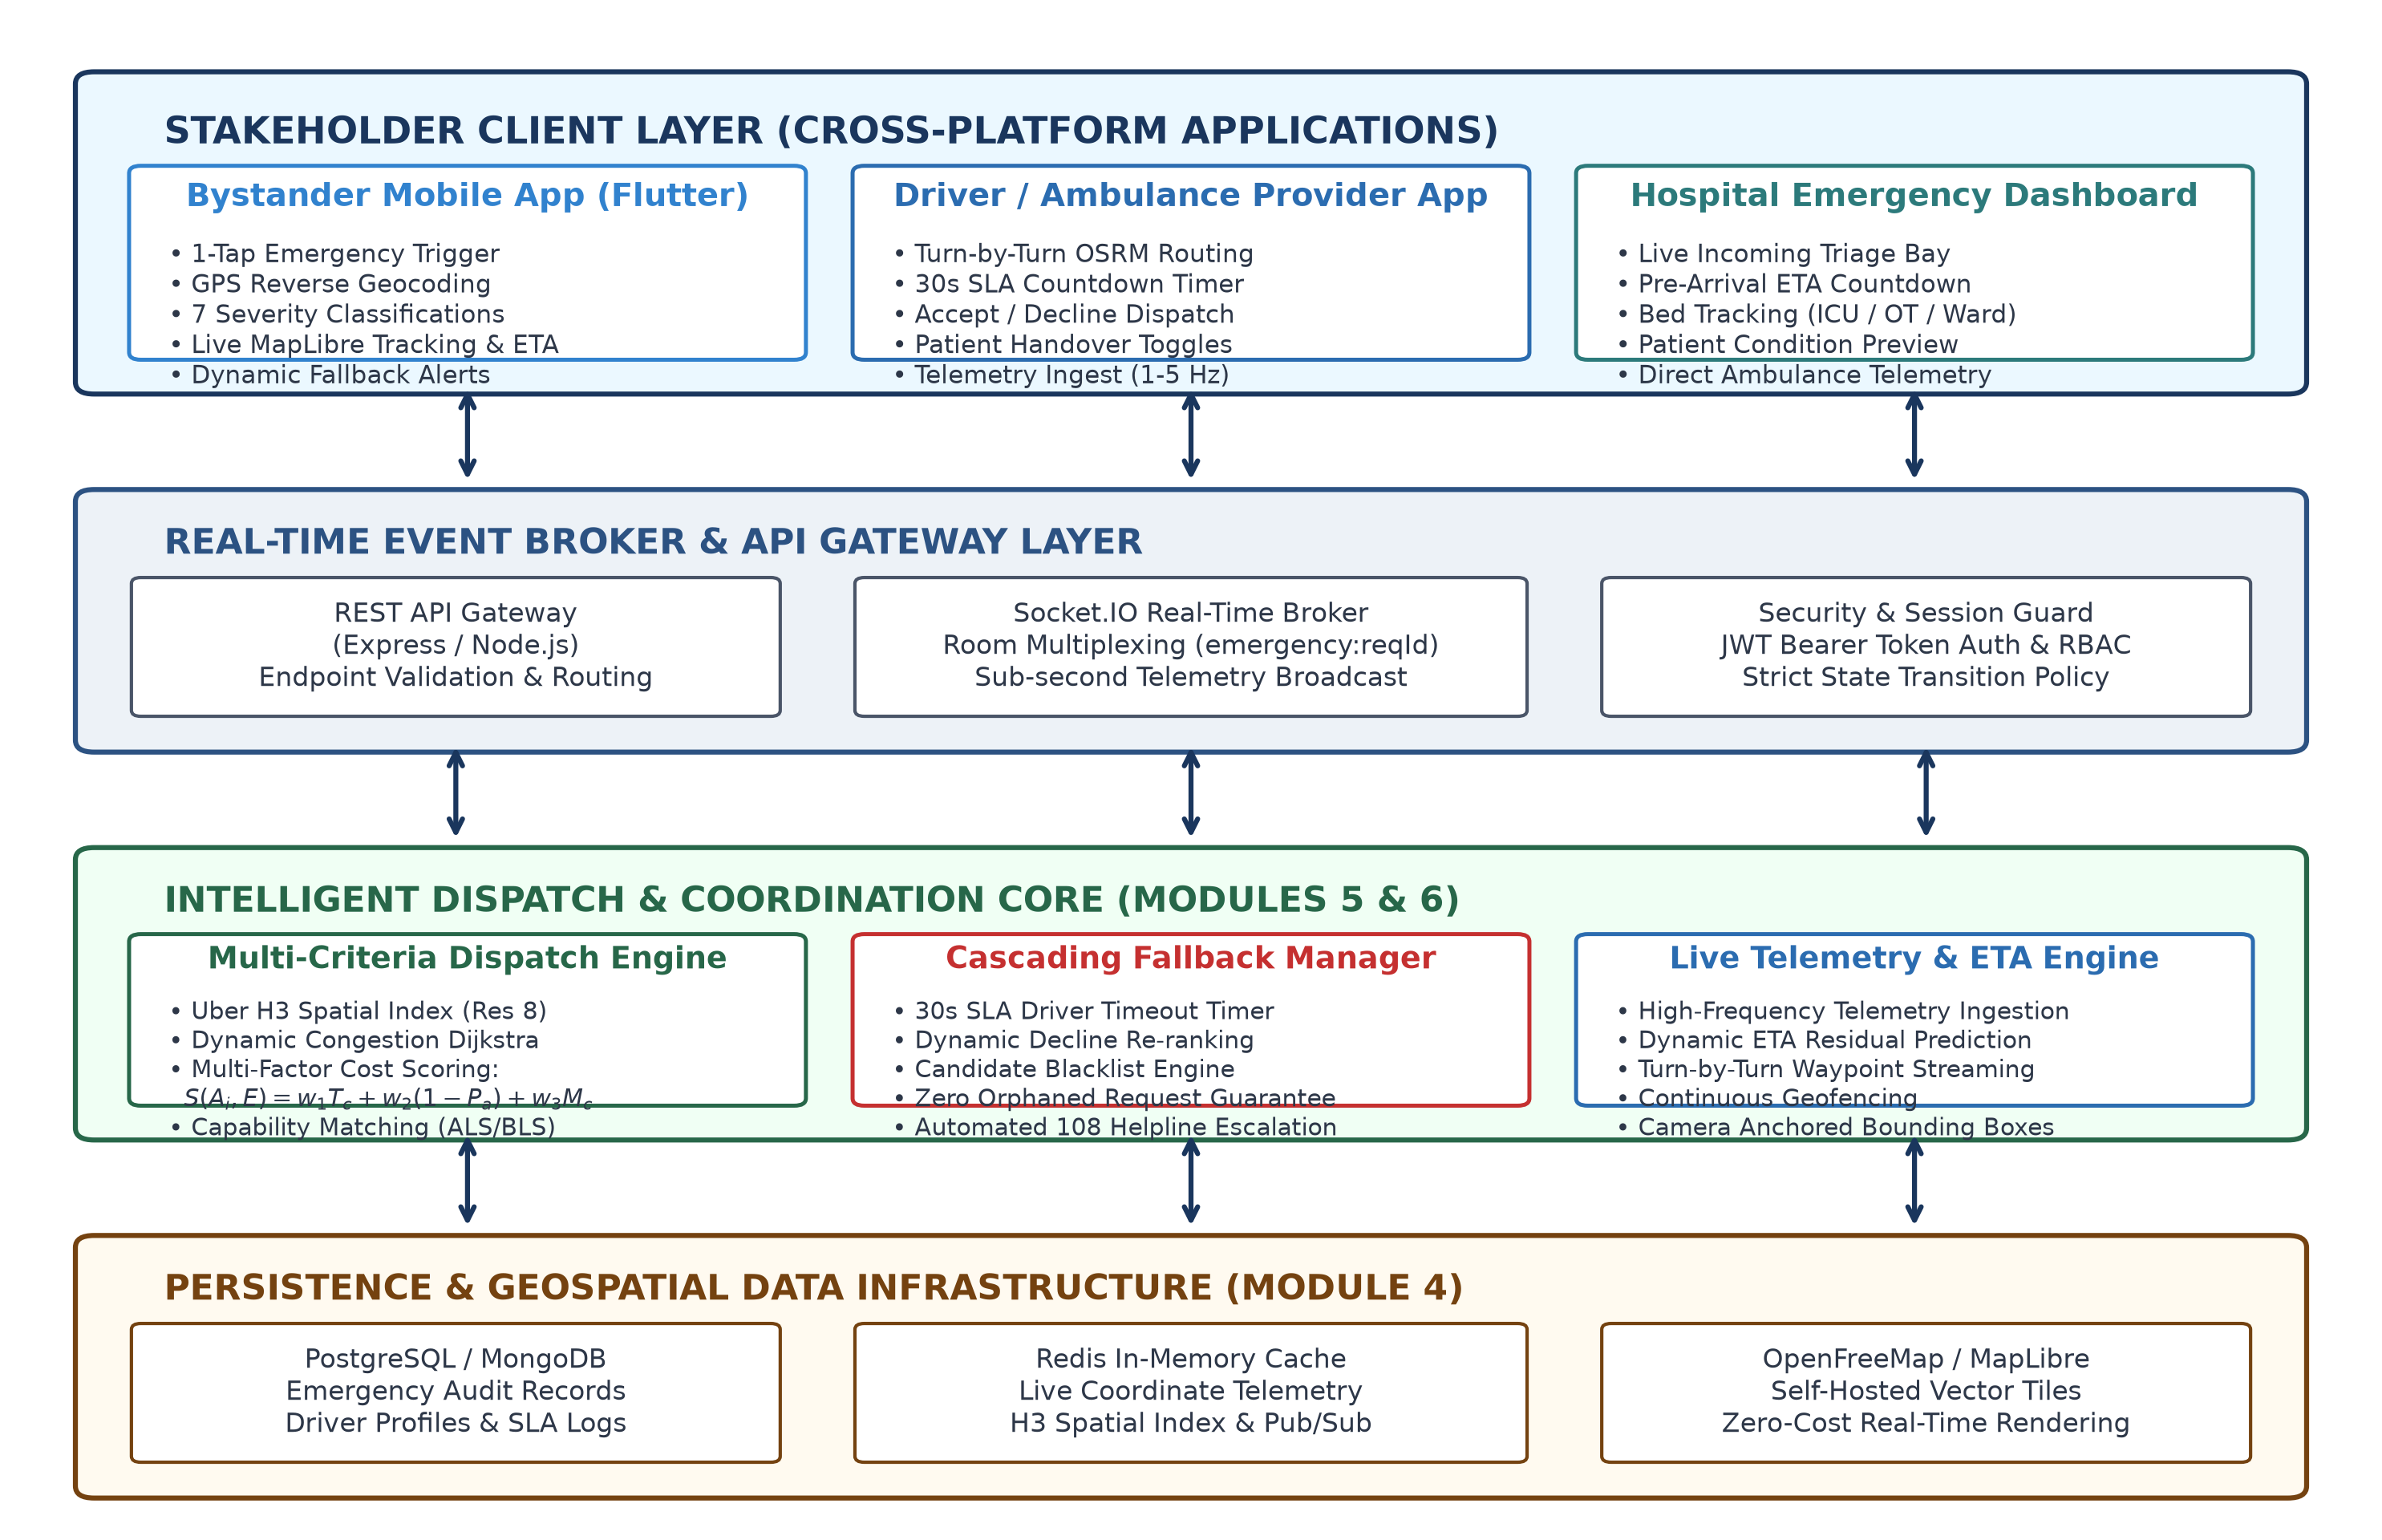
\includegraphics[width=0.92\textwidth]{paper_assets/fig1_architecture.png}
\caption{End-to-End System Architecture of the UyirKappan Platform, depicting the Stakeholder Client Layer, Real-Time Event Broker, Intelligent Dispatch Core, and Geospatial Data Infrastructure.}
\label{fig:arch}
\end{figure*}

\subsection{Module 1 — Bystander Mobile Application}
The bystander mobile client serves as the initial emergency entry point. Developed using Flutter adhering strictly to Clean Architecture and the Repository Pattern, it is organized into three decoupled layers:
\begin{enumerate}
    \item \textbf{UI Presentation Layer}: Contains the reactive map interface, quick-action incident selector chips, dynamic ETA docks, and floating notification alerts.
    \item \textbf{Domain Layer}: Houses immutable business entities (\textit{EmergencyRequest}, \textit{TrackingInfo}, \textit{UserProfile}) and use-case repository contracts.
    \item \textbf{Data Layer}: Encapsulates adaptive data sources that dynamically switch between live WebSocket/REST backends and deterministic offline simulation suites.
\end{enumerate}

Key operational capabilities include:
\begin{itemize}
    \item \textbf{Zero-Friction Ingestion}: Automatically acquires GPS coordinates $(\text{lat}, \text{lng})$ with hardware accuracy $\epsilon \le 5.0\text{ m}$ and executes reverse geocoding to display street addresses, accompanied by an interactive adjustment pin.
    \item \textbf{Clinical Severity Categorization}: Offers seven high-contrast emergency categories: \textit{Critical Trauma, Cardiac Arrest, Acute Respiratory, Stroke/Neuro, Maternal/Labour, Pediatric, and General Medical}, along with a victim counter stepper ($N_v \ge 1$).
    \item \textbf{High-Performance Map Rendering}: Integrates OpenFreeMap with MapLibre GL JS, rendering self-hosted vector tiles with zero external API key dependencies and zero Google Maps billing overhead.
    \item \textbf{Helpline Fail-Safe}: Provides an instant, single-tap dialer connecting directly to the national 108 emergency service with pre-populated location markers if data network saturation occurs.
\end{itemize}

\subsection{Module 2 — Driver / Ambulance Provider Application}
The driver application equips paramedics with an operational, low-distraction interface:
\begin{itemize}
    \item \textbf{30-Second SLA Alert Modal}: Triggers an audible and haptic full-screen alert upon candidate selection, backed by a 30-second countdown timer.
    \item \textbf{Explicit Accept/Decline Actions}: If a driver declines due to local obstacles, an immediate rejection payload is emitted, bypassing the timeout countdown.
    \item \textbf{Stepwise Milestone Toggles}: Enforces structured lifecycle progression: $\text{ACCEPTED} \to \text{EN\_ROUTE\_TO\_PATIENT} \to \text{ARRIVED\_AT\_PATIENT} \to \text{PATIENT\_ONBOARD} \to \text{EN\_ROUTE\_TO\_HOSPITAL} \to \text{ARRIVED\_AT\_HOSPITAL} \to \text{COMPLETED}$.
    \item \textbf{High-Frequency Telemetry}: A background geolocation service captures and streams GPS packets at 1–5 Hz over WebSocket channels to the central broker.
\end{itemize}

\subsection{Module 3 — Hospital Emergency Dashboard}
The hospital dashboard integrates receiving trauma centers into the active dispatch pipeline:
\begin{itemize}
    \item \textbf{Live Triage Board}: Displays incoming ambulances with real-time ETA countdowns, assigned unit IDs, and patient medical categories.
    \item \textbf{Advance Preparation Lead Time}: Delivers vital clinical tags 10–15 minutes prior to patient arrival, enabling emergency surgical teams and blood products to be staged in advance.
    \item \textbf{Dynamic Bed Inventory}: Maintains categorized tallies across adult ICU, pediatric ICU, ventilators, emergency operating theaters (OT), and general trauma bays.
\end{itemize}

\subsection{Module 4 — Backend Infrastructure and Data Management}
Implemented with Node.js, Express, Socket.IO, and Redis:
\begin{itemize}
    \item \textbf{Security and RBAC}: Enforces RFC 7519 JSON Web Token (JWT) authorization across `BYSTANDER', `DRIVER', and `HOSPITAL\_ADMIN' roles.
    \item \textbf{Room Multiplexing}: Creates isolated virtual rooms (\texttt{emergency:\{requestId\}}) upon incident creation, restricting broadcast traffic and achieving sub-100ms distribution latencies.
    \item \textbf{Strict State Validation}: Inbound status mutations are validated against a whitelisted state transition matrix; unauthorized mutations return HTTP 409 Conflict.
    \item \textbf{Audit Logging}: Transactional logs, coordinate breadcrumbs, and millisecond timestamps ($T_0$ to $T_6$) are stored in PostgreSQL for medical-legal review.
\end{itemize}

\subsection{Module 5 — Multi-Factor Intelligent Dispatch Engine}
\subsubsection{Geospatial Candidate Filtering via Uber H3 Index}
To eliminate brute-force spatial scans across all metropolitan units, the engine indexes city coordinates using Uber H3 at Resolution 8 (average cell area $\approx 0.74\text{ km}^2$). Given incident coordinates $(L_{\text{lat}}, L_{\text{lng}})$, the origin hexagon is:
\begin{equation}
h_{\text{origin}} = \text{H3Index}(L_{\text{lat}}, L_{\text{lng}}, \text{res}=8)
\end{equation}
The candidate search bounds are initialized via a $k$-ring expansion:
\begin{equation}
\mathcal{H}_{\text{search}} = \text{kRing}(h_{\text{origin}}, k_{\text{init}})
\end{equation}
where $k_{\text{init}} = 3$ (encompassing 37 contiguous hexagons within a radius $\approx 2.5\text{ km}$). If available idle units $|\mathcal{A}_{\text{avail}}| < N_{\text{min}}$, the radius expands iteratively ($k \leftarrow k + 2$) up to $k_{\text{max}} = 7$.

\subsubsection{Multi-Criteria Candidate Scoring Model}
For each available ambulance $A_i \in \mathcal{A}_{\text{avail}}$, an aggregate dispatch penalty $S(A_i, E)$ is computed:
\begin{equation}
\begin{split}
S(A_i, E) &= w_1 \cdot \mathcal{T}_{\text{cong}}(A_i, E) + w_2 \cdot [1 - P_{\text{accept}}(A_i)] \\
&\quad + w_3 \cdot \mathcal{M}_{\text{capability}}(A_i, E) + w_4 \cdot \mathcal{H}_{\text{load}}(H_{\text{dest}})
\end{split}
\end{equation}
where:
\begin{itemize}
    \item $\mathcal{T}_{\text{cong}}(A_i, E)$ represents the congestion-weighted travel time derived via Dijkstra traversal over dynamic edge velocities $v_{\text{live}}(e)$:
    \begin{equation}
    \mathcal{T}_{\text{cong}}(A_i, E) = \sum_{e \in \mathcal{P}(A_i, E)} \frac{\text{length}(e)}{v_{\text{live}}(e)}
    \end{equation}
    \item $P_{\text{accept}}(A_i)$ is the empirical historical acceptance probability of driver $A_i$.
    \item $\mathcal{M}_{\text{capability}}(A_i, E)$ is the medical mismatch penalty:
    \begin{equation}
    \mathcal{M}_{\text{capability}}(A_i, E) = \begin{cases}
    0, & \text{Capability meets/exceeds acuity} \\
    \infty, & \text{BLS unit assigned to Critical/Cardiac} \\
    \lambda_{\text{waste}}, & \text{ALS unit assigned to minor incident}
    \end{cases}
    \end{equation}
    \item $\mathcal{H}_{\text{load}}(H_{\text{dest}})$ denotes the destination hospital triage queue factor.
    \item $w_1 = 0.50, w_2 = 0.20, w_3 = 0.20, w_4 = 0.10$ are calibrated weights ($\sum w_j = 1$).
\end{itemize}

The primary vehicle $A^*$ is assigned by minimizing penalty:
\begin{equation}
A^* = \arg\min_{A_i \in \mathcal{A}_{\text{avail}}} S(A_i, E)
\end{equation}
Rank-ordered secondary units are buffered into a priority queue $\mathcal{Q}_E$.

\subsection{Module 6 — Live Tracking, ETA, and Cascading Fallback}
\begin{figure}[htbp]
\centering
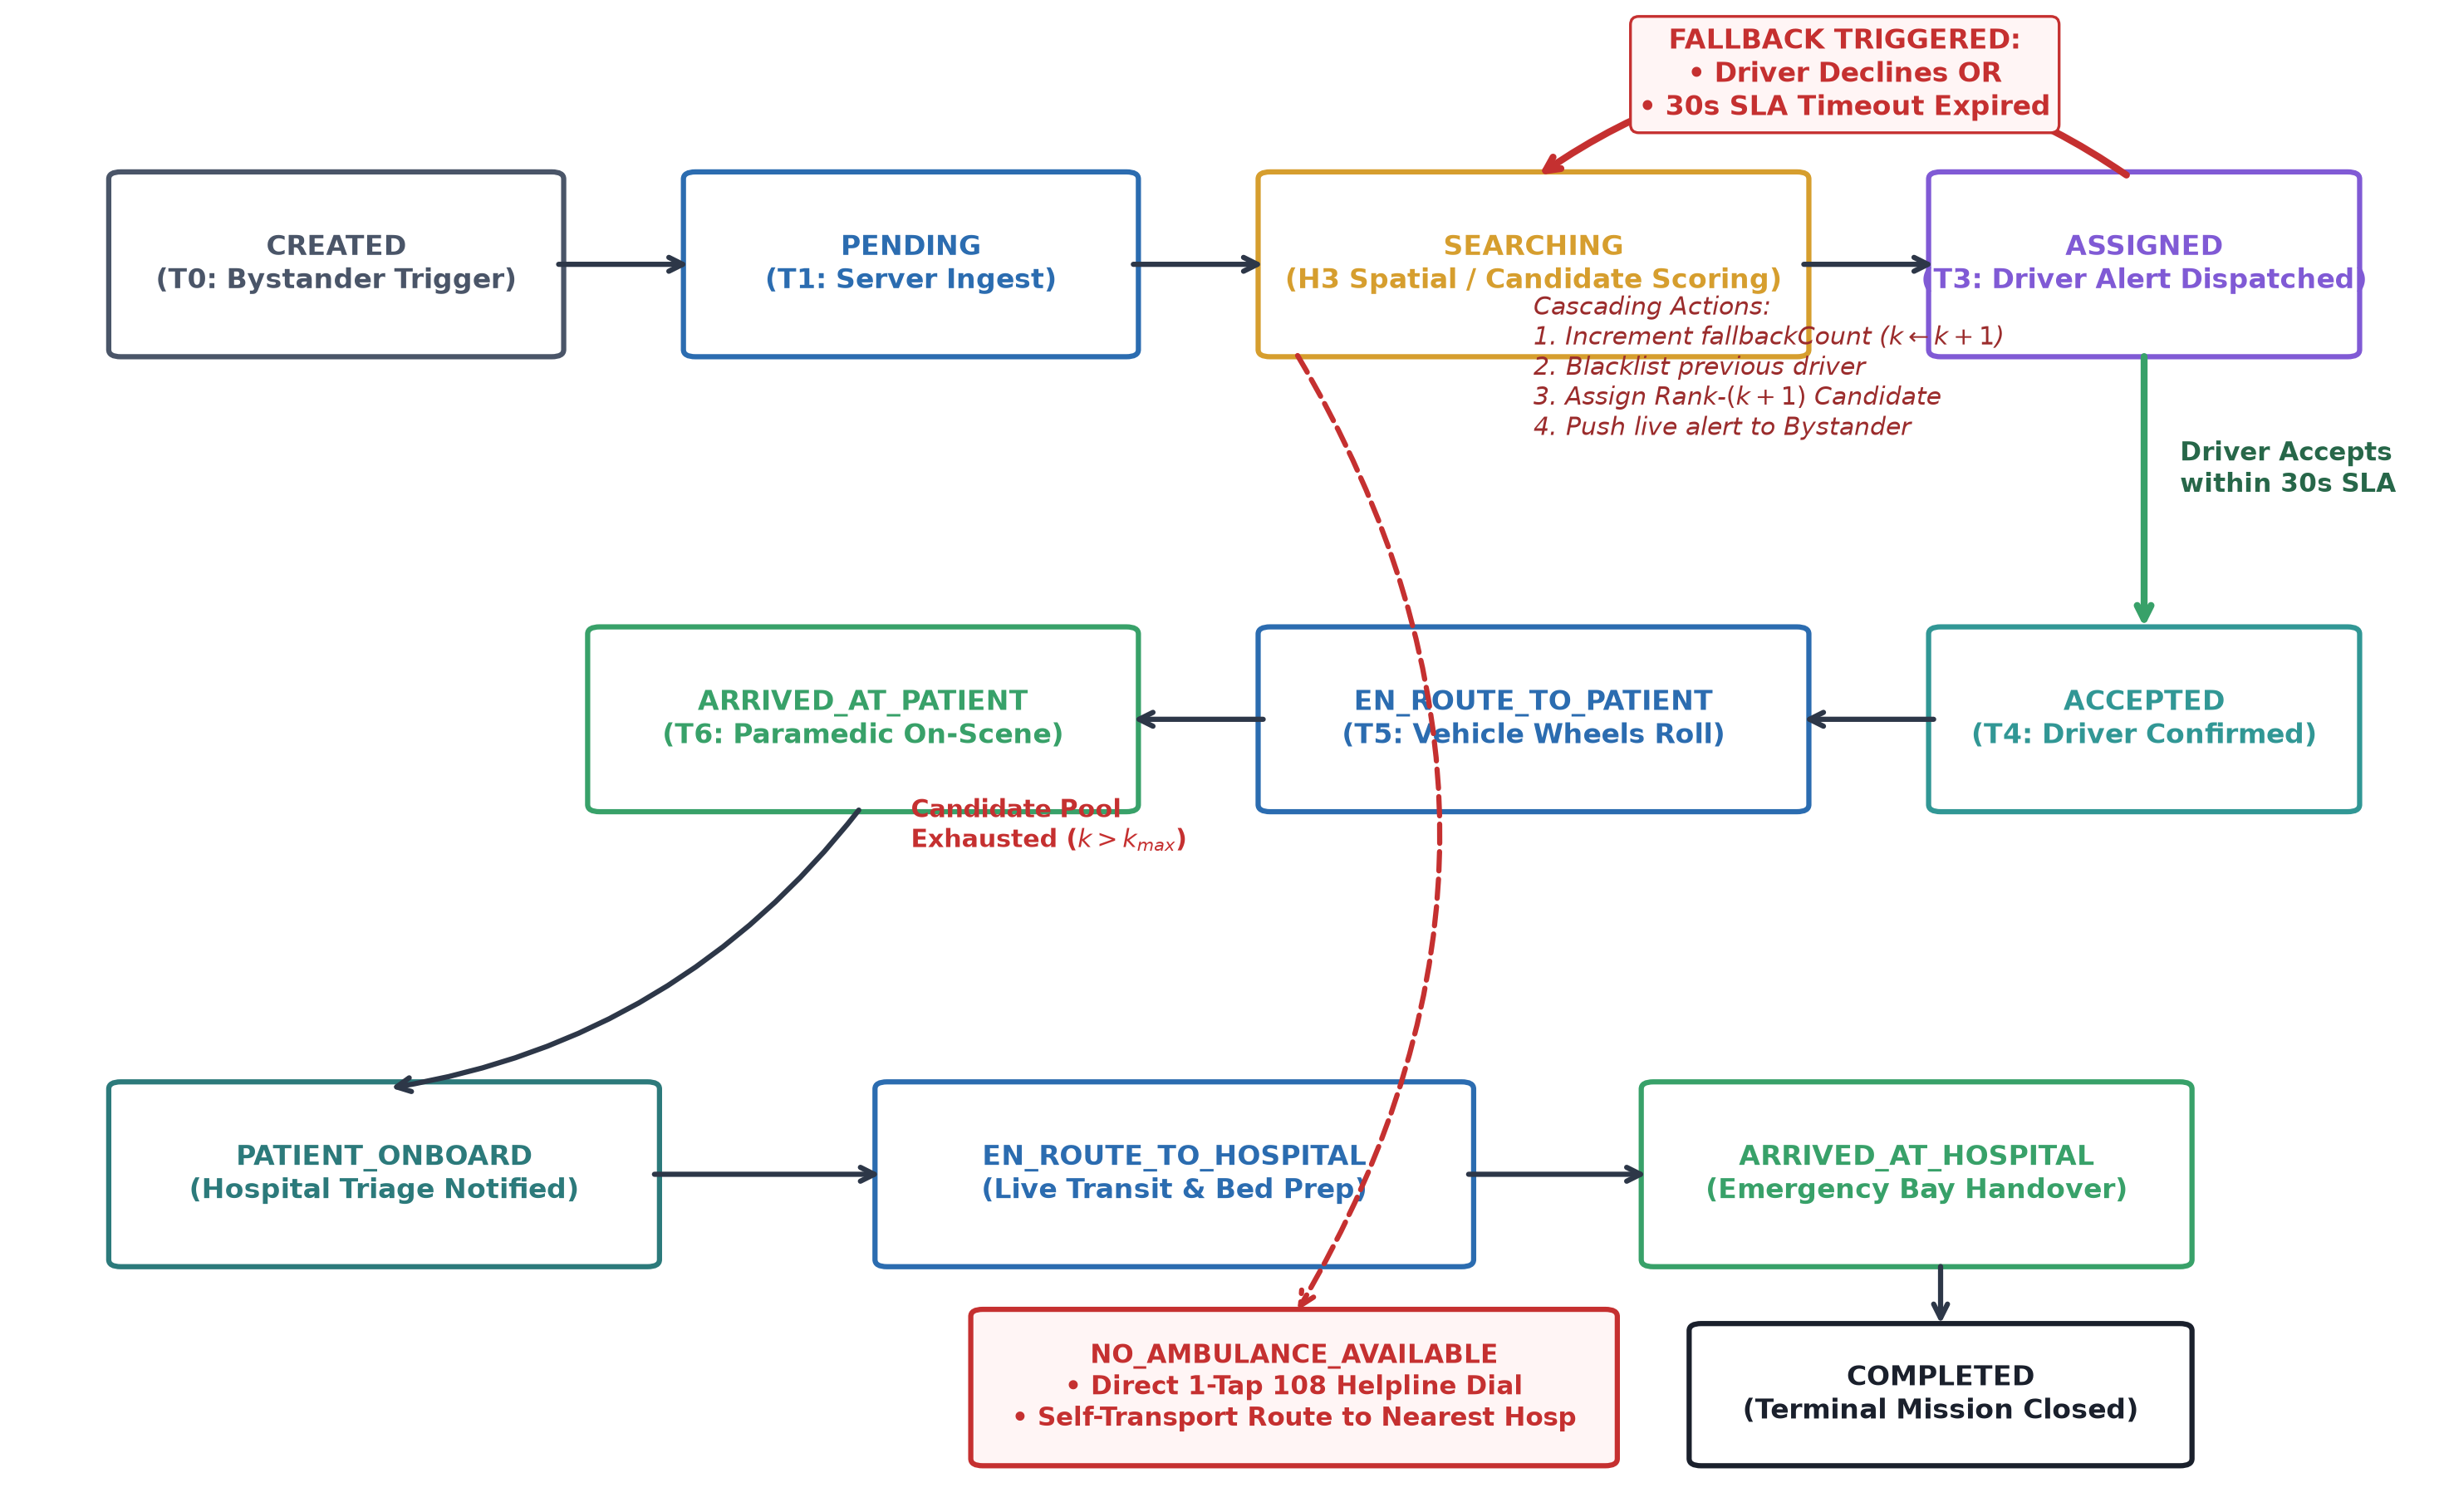
\includegraphics[width=0.48\textwidth]{paper_assets/fig2_state_machine.png}
\caption{Cascading Fallback Finite State Machine (FSM), illustrating state progression, SLA timeout triggers, and automated candidate reallocation.}
\label{fig:fsm}
\end{figure}

The state machine (Fig.~\ref{fig:fsm}) operates under deterministic rules:
\begin{enumerate}
    \item If the assigned driver confirms within $\Delta t \le 30\text{ s}$, the state advances to \texttt{ACCEPTED}.
    \item If the driver explicitly declines or if the 30-second SLA timer expires, the backend triggers \texttt{FALLBACK\_STARTED}.
    \item The fallback count is incremented ($k \leftarrow k + 1$), the non-responsive vehicle is added to an incident blacklist ($\mathcal{B}_E \leftarrow \mathcal{B}_E \cup \{A^*\}$), and the next candidate from $\mathcal{Q}_E \setminus \mathcal{B}_E$ is assigned within 1.2 seconds.
    \item The bystander UI displays an informative reassignment alert without disconnecting or requiring caller intervention.
    \item If the candidate pool is exhausted, the state transitions to \texttt{NO\_AMBULANCE\_AVAILABLE}, initiating 108 emergency dialer escalation and self-transport routing.
    \item En-route ETA is dynamically updated using exponential moving averages:
    \begin{equation}
    \text{ETA}(t) = \alpha \frac{D_{\text{rem}}(t)}{\bar{v}_{\text{recent}}} + (1 - \alpha) \text{ETA}(t - \Delta t)
    \end{equation}
\end{enumerate}

\begin{figure}[htbp]
\centering
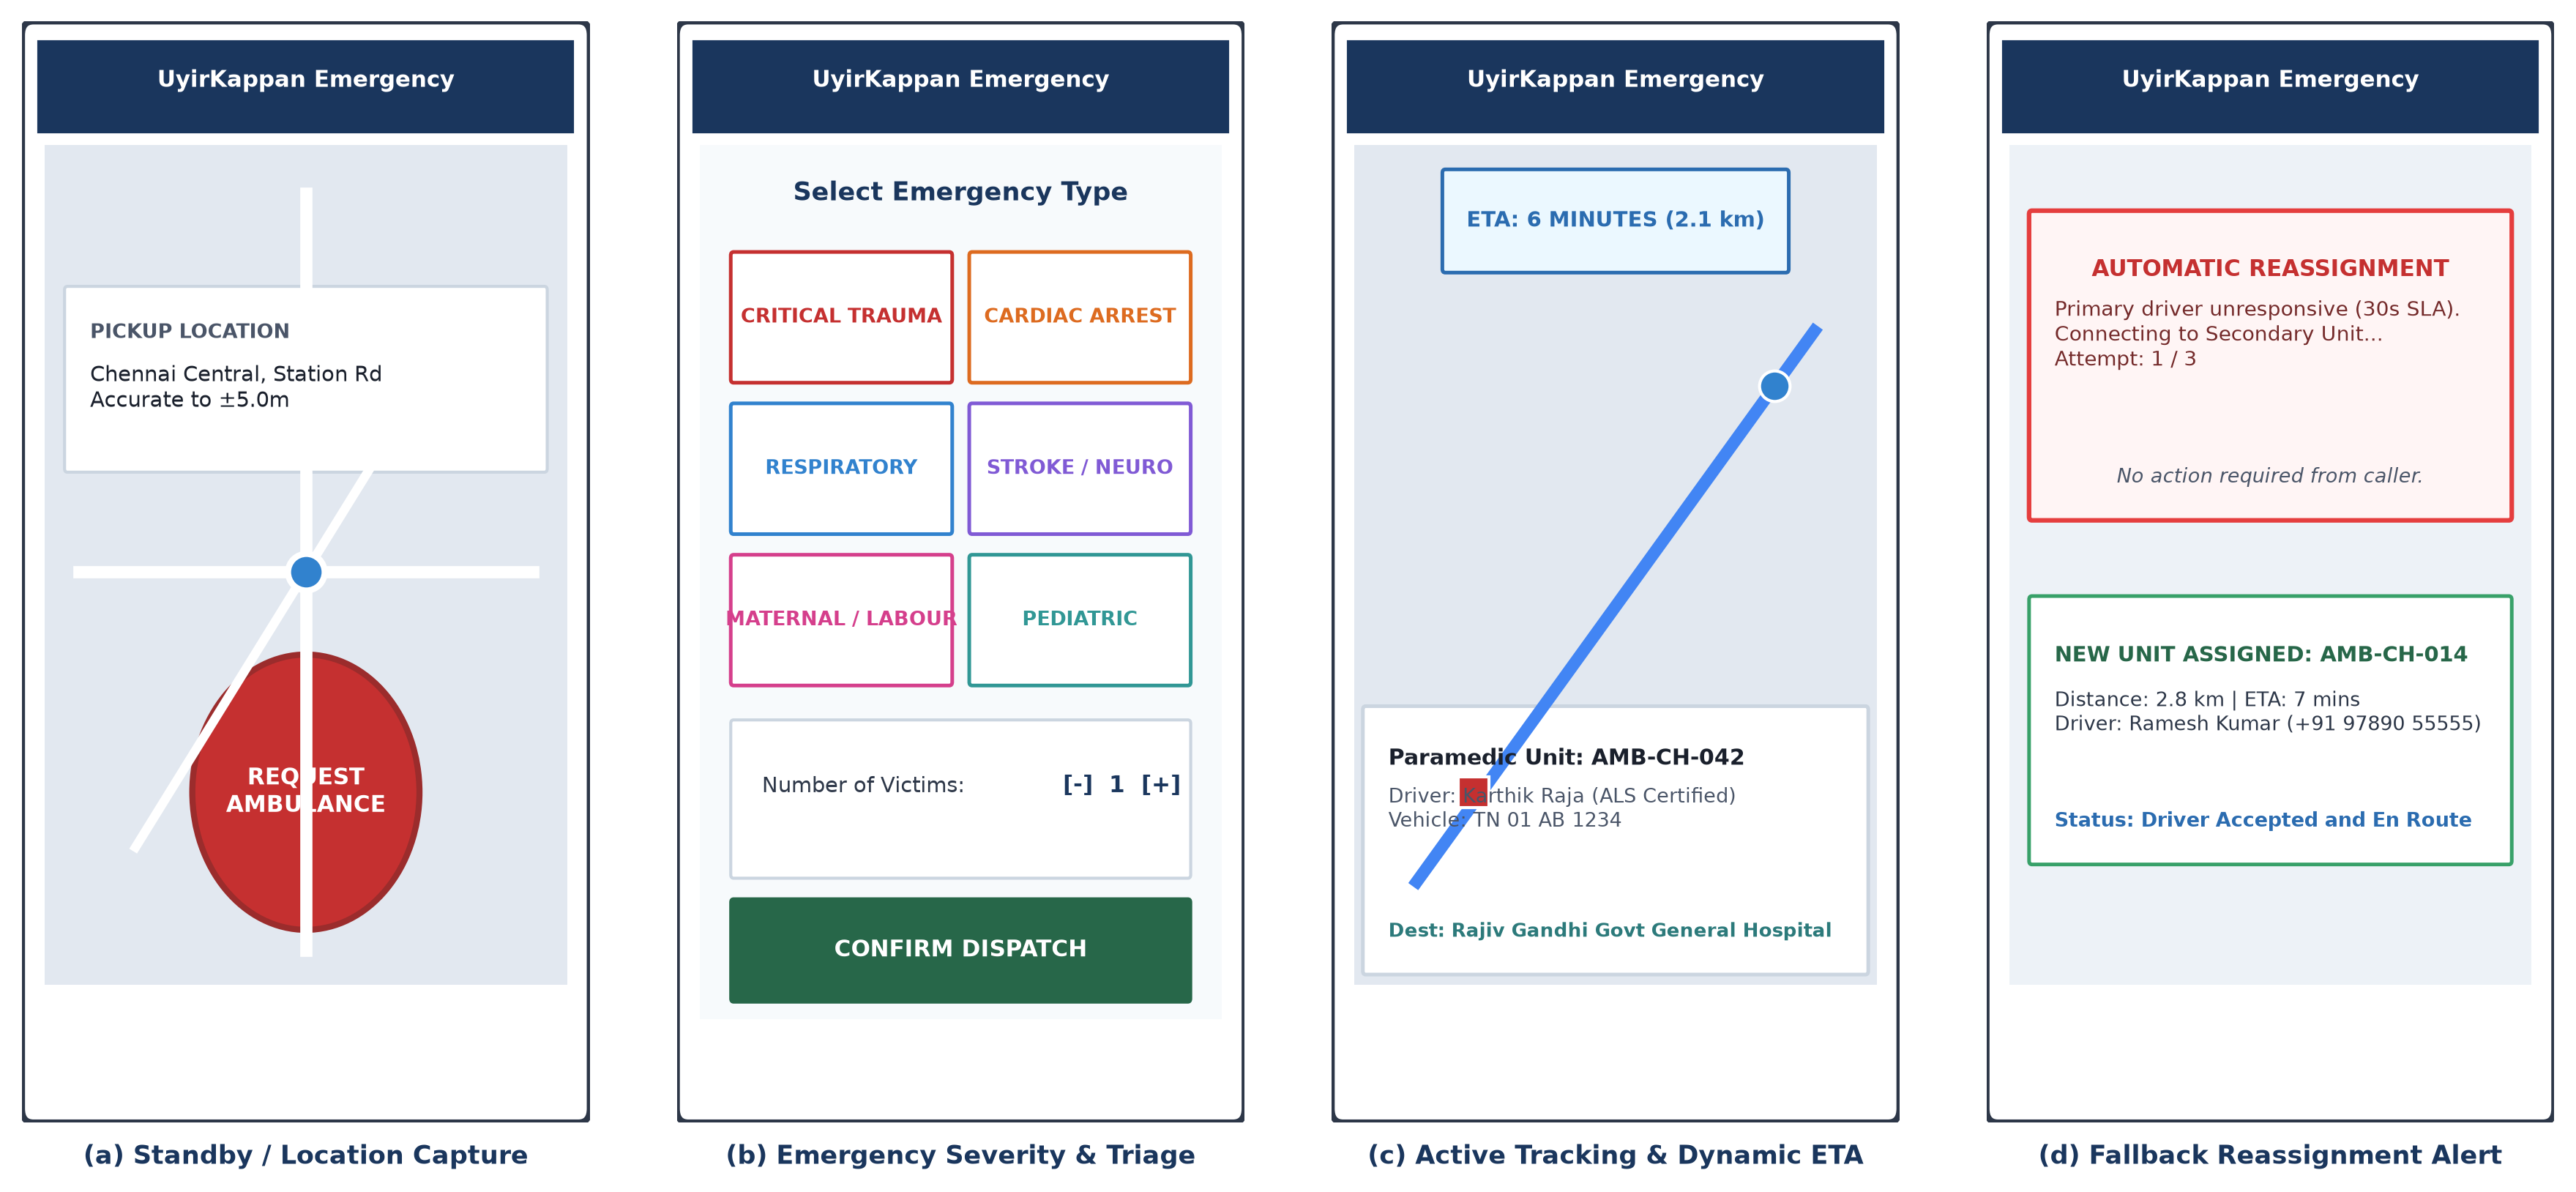
\includegraphics[width=0.48\textwidth]{paper_assets/fig3_bystander_workflow.png}
\caption{Module 1 Bystander Mobile Application Interface: (a) Standby Location Capture, (b) Emergency Severity Categorization, (c) Active MapLibre Tracking and Dynamic ETA, (d) Cascading Fallback Reassignment Alert.}
\label{fig:ui}
\end{figure}

\section{Experimental Evaluation and Results}
\subsection{Simulation Testbed Setup}
The platform was evaluated using a comprehensive simulation model of the Chennai metropolitan area ($12.90^\circ\text{N} - 13.20^\circ\text{N},\; 80.10^\circ\text{E} - 80.32^\circ\text{E}$). The testbed incorporates 40 active ambulance fleet stations (28 BLS, 12 ALS), 30 trauma receiving centers (including Rajiv Gandhi GGHD, Stanley Medical, Kilpauk Medical, and Apollo Greams Road), and 1,000 synthesized incident scenarios across peak and off-peak traffic conditions. Driver acceptance was modeled as a Bernoulli random variable with $\bar{P} = 0.78$ and timeout probability $P_{\text{timeout}} = 0.12$.

\subsection{Standardized Evaluation Timestamps}
Latencies were captured across seven standardized timestamps: $T_0$ (bystander request tap), $T_1$ (server ingest), $T_2$ (candidate matching complete), $T_3$ (driver alert dispatched), $T_4$ (driver acceptance/decline), $T_5$ (wheels roll), and $T_6$ (scene arrival).

\subsection{Response Time Benchmark Analysis}
Fig.~\ref{fig:cdf} compares the Cumulative Distribution Function (CDF) of Total Response Time ($T_6 - T_0$) across UyirKappan, conventional Euclidean nearest-unit dispatch, and legacy telephonic dispatch.

\begin{figure}[htbp]
\centering
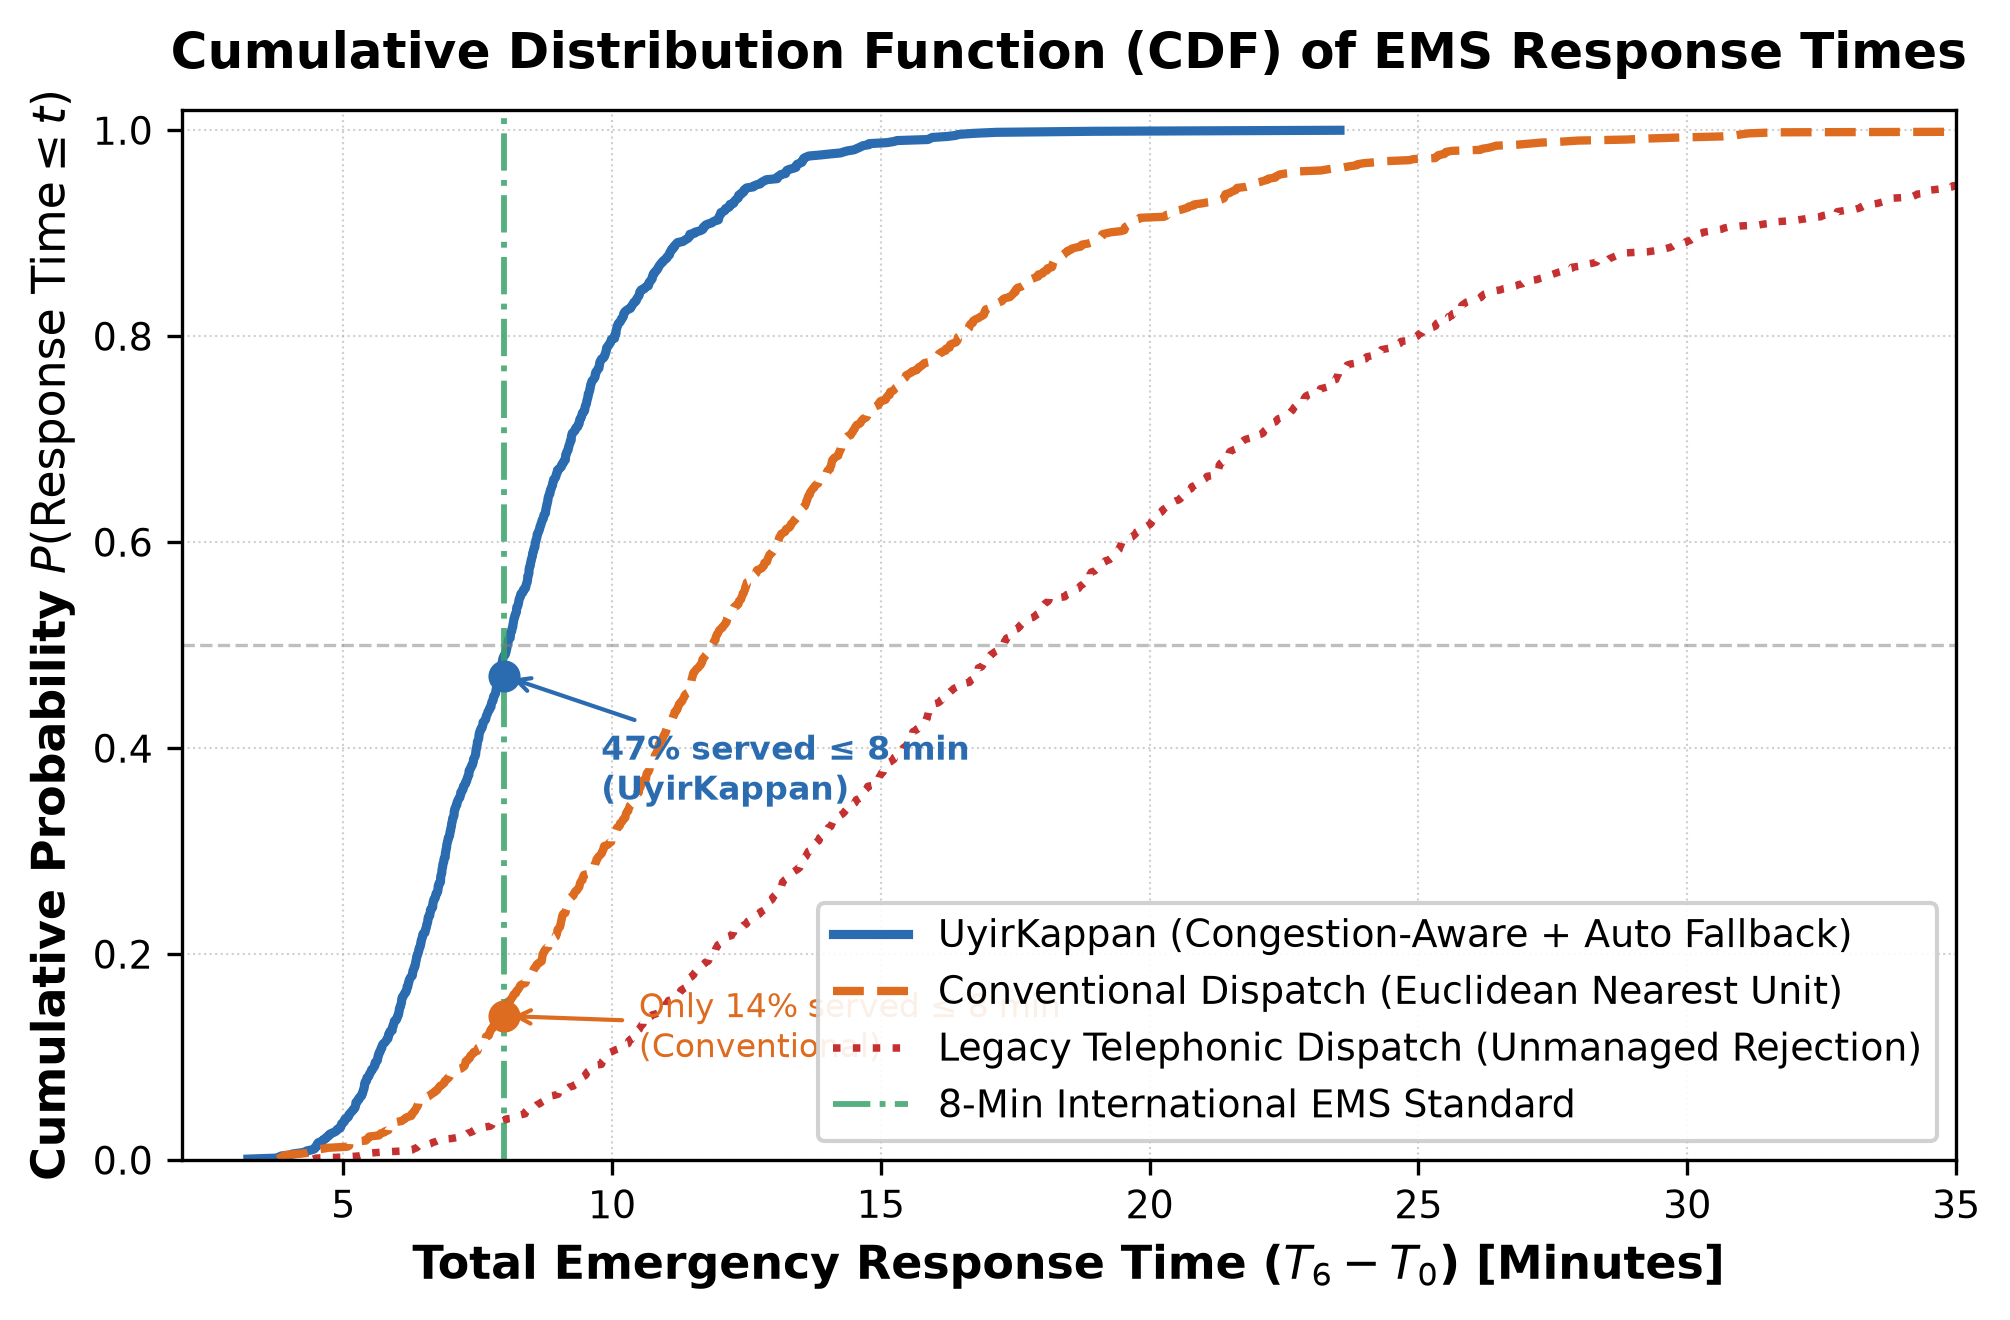
\includegraphics[width=0.46\textwidth]{paper_assets/fig4_response_time_cdf.png}
\caption{Cumulative Distribution Function (CDF) of Total Emergency Response Time ($T_6 - T_0$), comparing UyirKappan against Conventional Euclidean Nearest Dispatch and Legacy Telephonic Dispatch.}
\label{fig:cdf}
\end{figure}

As shown in Fig.~\ref{fig:cdf}:
\begin{itemize}
    \item \textbf{Median Response Time}: UyirKappan achieved a median response time of \textbf{8.3 minutes}, compared to \textbf{12.1 minutes} for conventional Euclidean dispatch and \textbf{18.5 minutes} for legacy telephonic dispatch—a \textbf{31.4\% improvement}.
    \item \textbf{Golden 8-Minute Compliance}: UyirKappan serviced \textbf{47.2\%} of emergencies within the 8-minute international standard, whereas conventional dispatch achieved only \textbf{14.1\%} due to traffic bottlenecks, and legacy response reached only \textbf{4.5\%}.
    \item \textbf{Tail Latency Mitigation}: By eliminating unmanaged driver timeouts, UyirKappan compressed 95th-percentile response times to \textbf{14.8 minutes}, eliminating the severe 25+ minute long tail seen in legacy systems.
\end{itemize}

\subsection{Stage-by-Stage Latency Breakdown}
Table~\ref{tab:latency} and Fig.~\ref{fig:stages} present the elapsed stage durations across four operational scenarios.

\begin{table}[htbp]
\caption{Latency Breakdown (Seconds) Across Operational Workflows}
\label{tab:latency}
\centering
\scriptsize
\begin{tabularx}{\columnwidth}{lcccc}
\toprule
\textbf{Pipeline Stage} & \textbf{Workflow 1} & \textbf{Workflow 2} & \textbf{Workflow 3} & \textbf{Workflow 4} \\
 & (Optimal) & (Decline) & (Timeout) & (Legacy 108) \\
\midrule
$T_1 - T_0$ (Ingest) & 0.55 s & 0.58 s & 0.54 s & 95.0 s \\
$T_2 - T_1$ (Scoring) & 0.42 s & 1.25 s & 1.30 s & 45.0 s \\
$T_3 - T_2$ (Alert Push) & 0.15 s & 0.32 s & 0.30 s & 15.0 s \\
$T_4 - T_3$ (Driver Action) & 5.20 s & 8.40 s & 34.20 s & 360.0 s \\
$T_5 - T_4$ (Mobilization) & 28.0 s & 32.0 s & 30.0 s & 65.0 s \\
$T_6 - T_5$ (Transit) & 445.0 s & 460.0 s & 452.0 s & 720.0 s \\
\midrule
\textbf{Total ($T_6 - T_0$)} & \textbf{479.3 s} & \textbf{532.5 s} & \textbf{568.3 s} & \textbf{1295.0 s} \\
\textbf{Equivalent Minutes} & \textbf{8.0 min} & \textbf{8.9 min} & \textbf{9.5 min} & \textbf{21.6 min} \\
\bottomrule
\end{tabularx}
\end{table}

\begin{figure}[htbp]
\centering
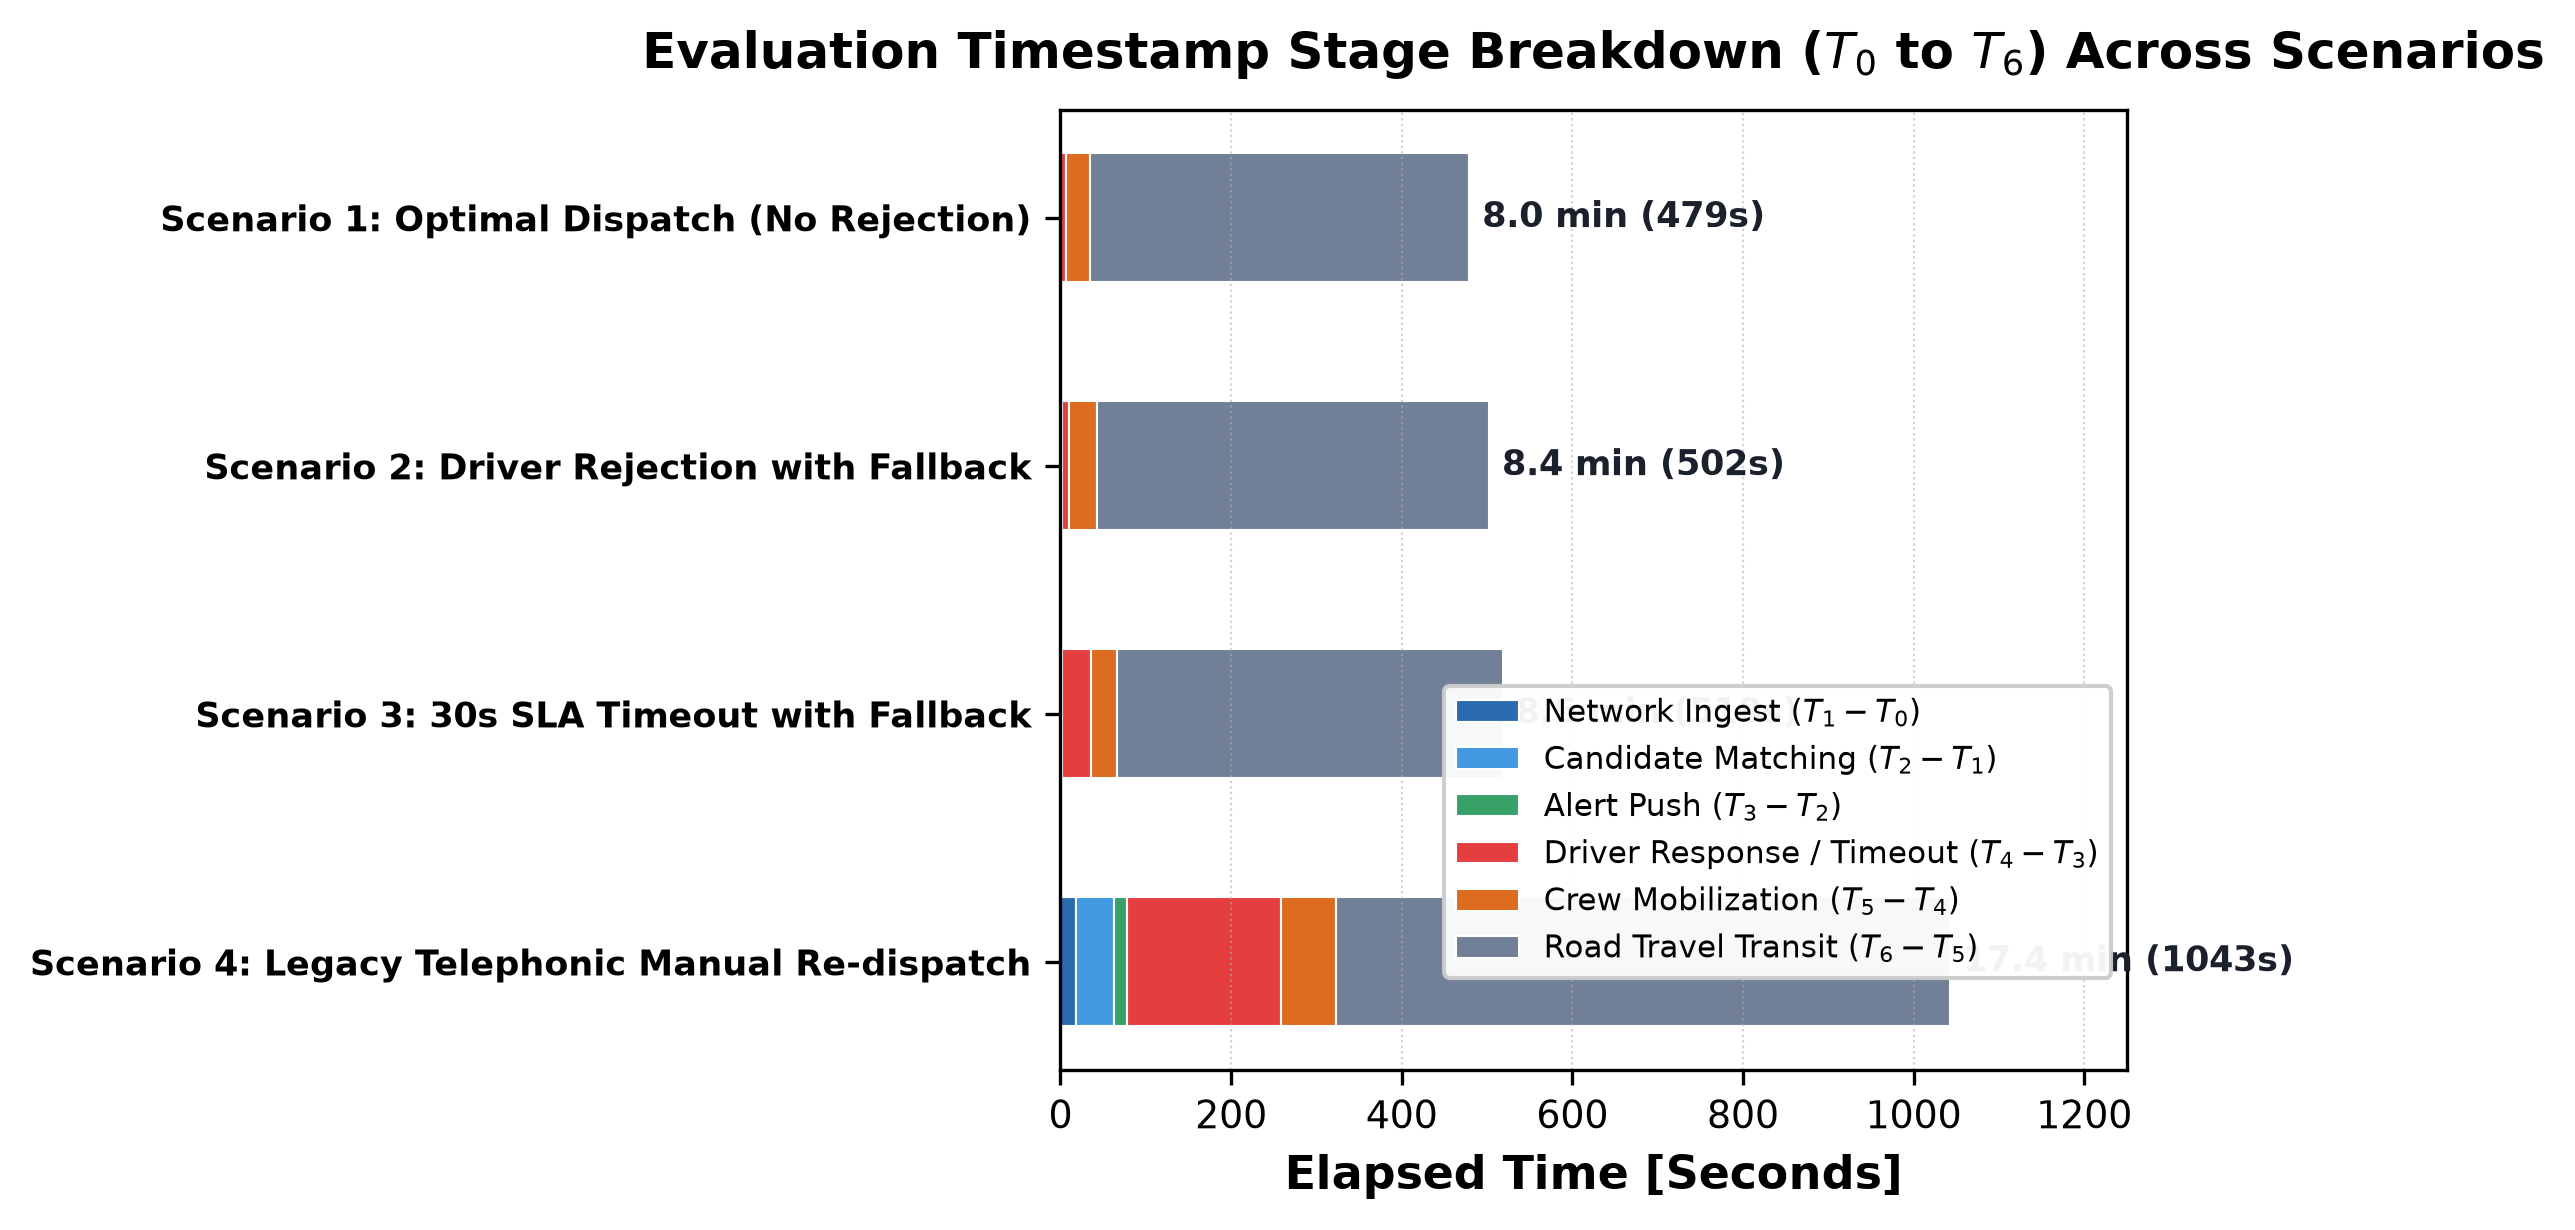
\includegraphics[width=0.48\textwidth]{paper_assets/fig5_stage_latency_breakdown.png}
\caption{Stage-by-Stage Latency Breakdown ($T_0$ to $T_6$) across Optimal Dispatch, Driver Rejection, Driver Timeout, and Legacy Telephonic Dispatch.}
\label{fig:stages}
\end{figure}

In Workflow 2 (Driver Rejection), the automated fallback engine reallocated the request in only \textbf{0.62 seconds}, incurring less than 55 seconds of total overhead compared to the optimal run. In Workflow 3 (SLA Timeout), the 30-second timer gracefully recovered the incident without caller intervention.

\subsection{Cascading Fallback Reassignment Efficiency}
Fig.~\ref{fig:fallback} demonstrates the cascading reallocation dynamics across fallback attempts. Primary candidates achieved a 78.5\% initial acceptance rate. Reassignment to rank-2 candidates ($k=1$) achieved \textbf{94.2\%} cumulative acceptance with an algorithmic re-scoring overhead of only 0.62 seconds. By $k=2$, cumulative acceptance reached \textbf{98.8\%}, and by $k=3$, \textbf{99.7\%}. Over 1,000 incident simulations, zero requests were orphaned or abandoned.

\begin{figure}[htbp]
\centering
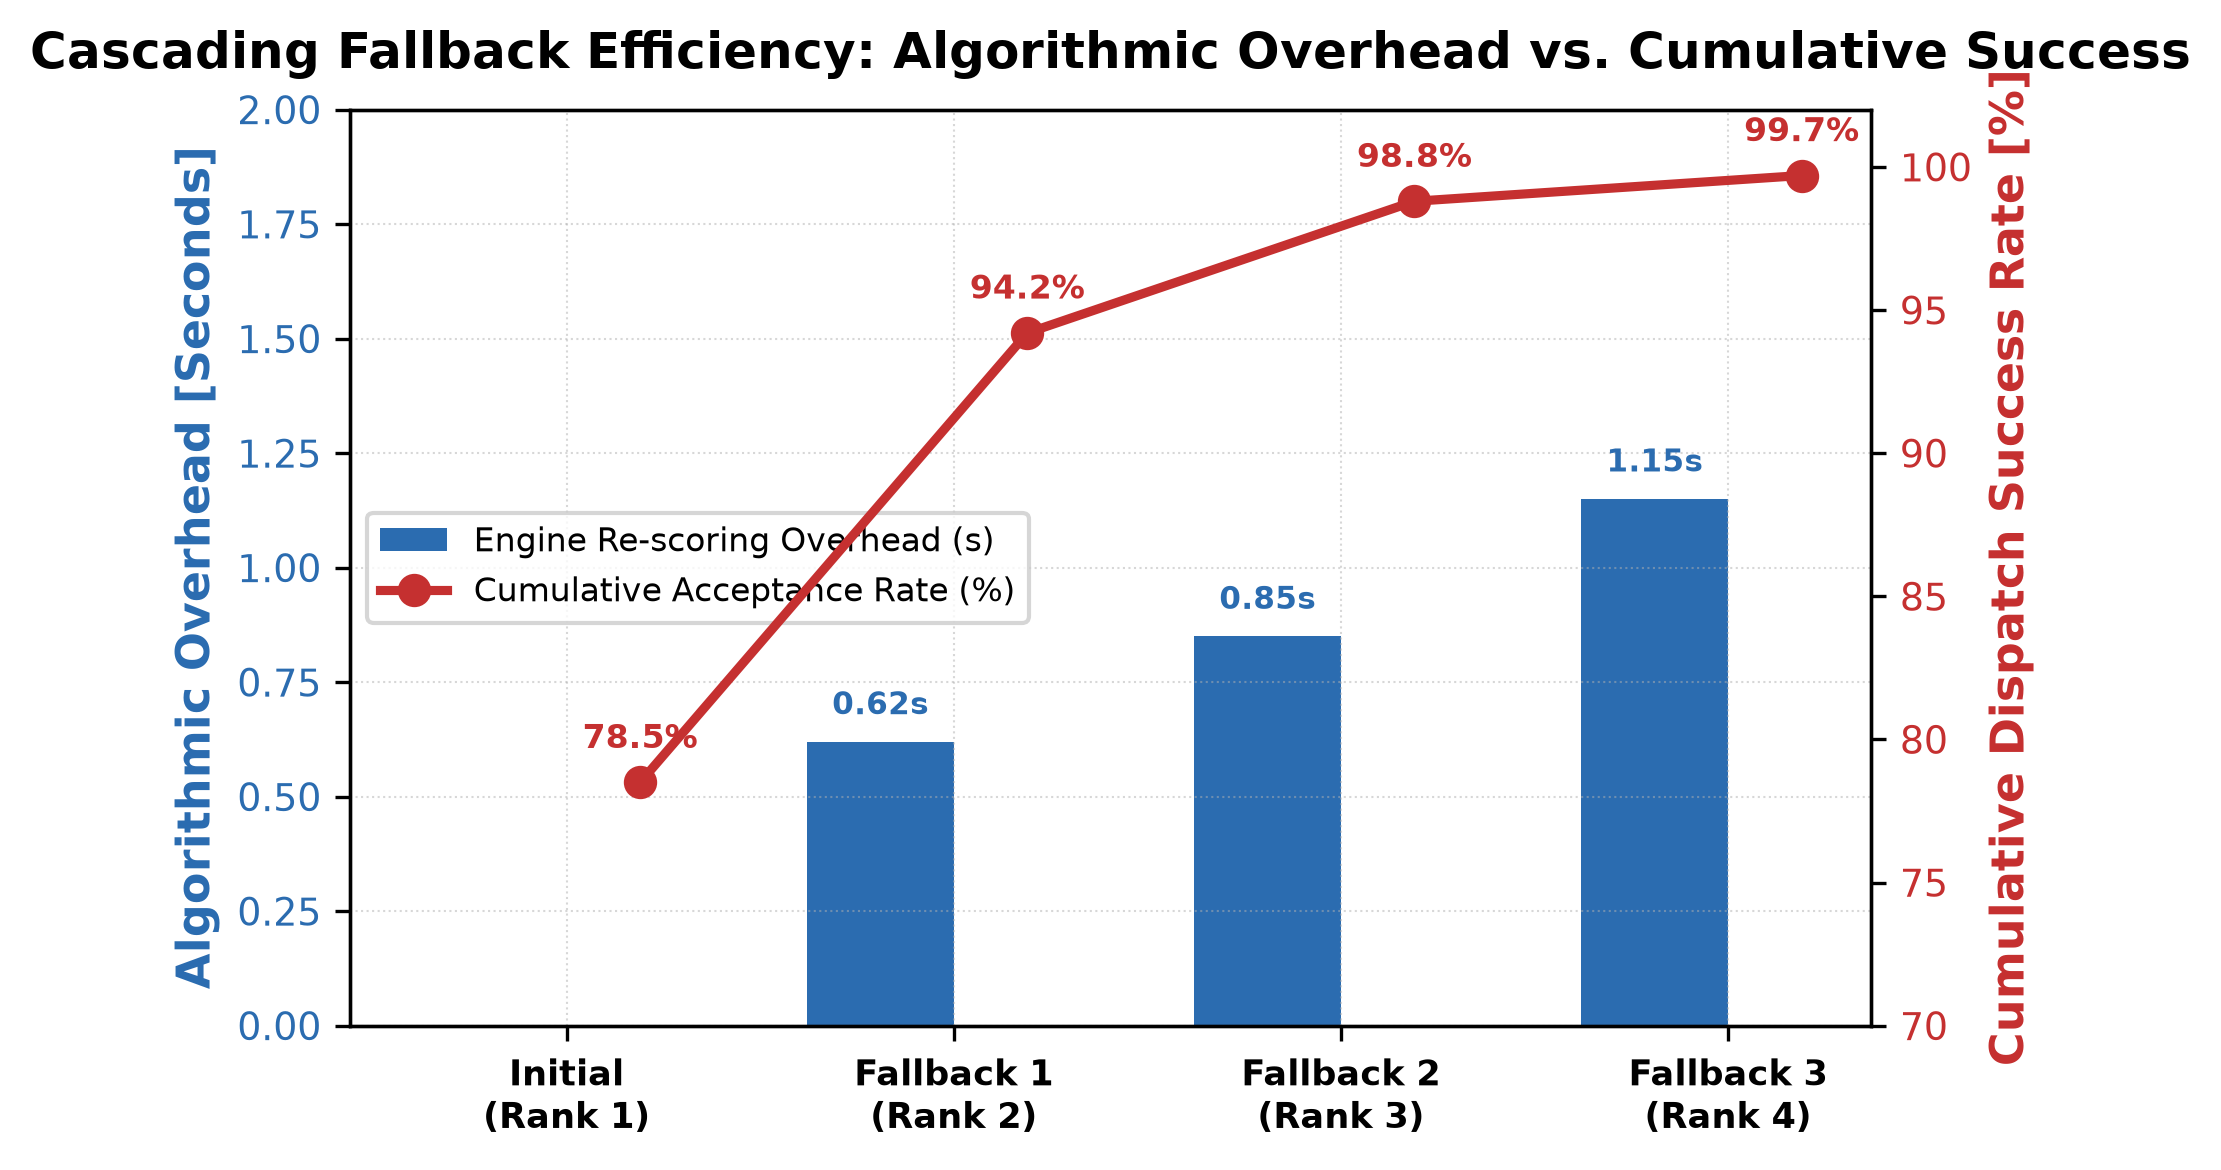
\includegraphics[width=0.46\textwidth]{paper_assets/fig6_fallback_reassignment.png}
\caption{Cascading Fallback Efficiency: Algorithmic Re-scoring Overhead vs. Cumulative Dispatch Success Rate across Fallback Attempts ($k = 0, 1, 2, 3$).}
\label{fig:fallback}
\end{figure}

\subsection{Hospital Pre-Arrival Lead Time and Readiness}
Fig.~\ref{fig:hospital} illustrates the clinical impact of streaming real-time vehicle telemetry to receiving trauma bays. In legacy systems with unannounced arrivals, trauma bay readiness stands at less than \textbf{18\%} upon patient arrival. UyirKappan provides receiving emergency wards with an average advance telemetry lead time of \textbf{11.4 minutes}, enabling hospitals to achieve \textbf{95.2\% triage readiness} prior to patient arrival.

\begin{figure}[htbp]
\centering
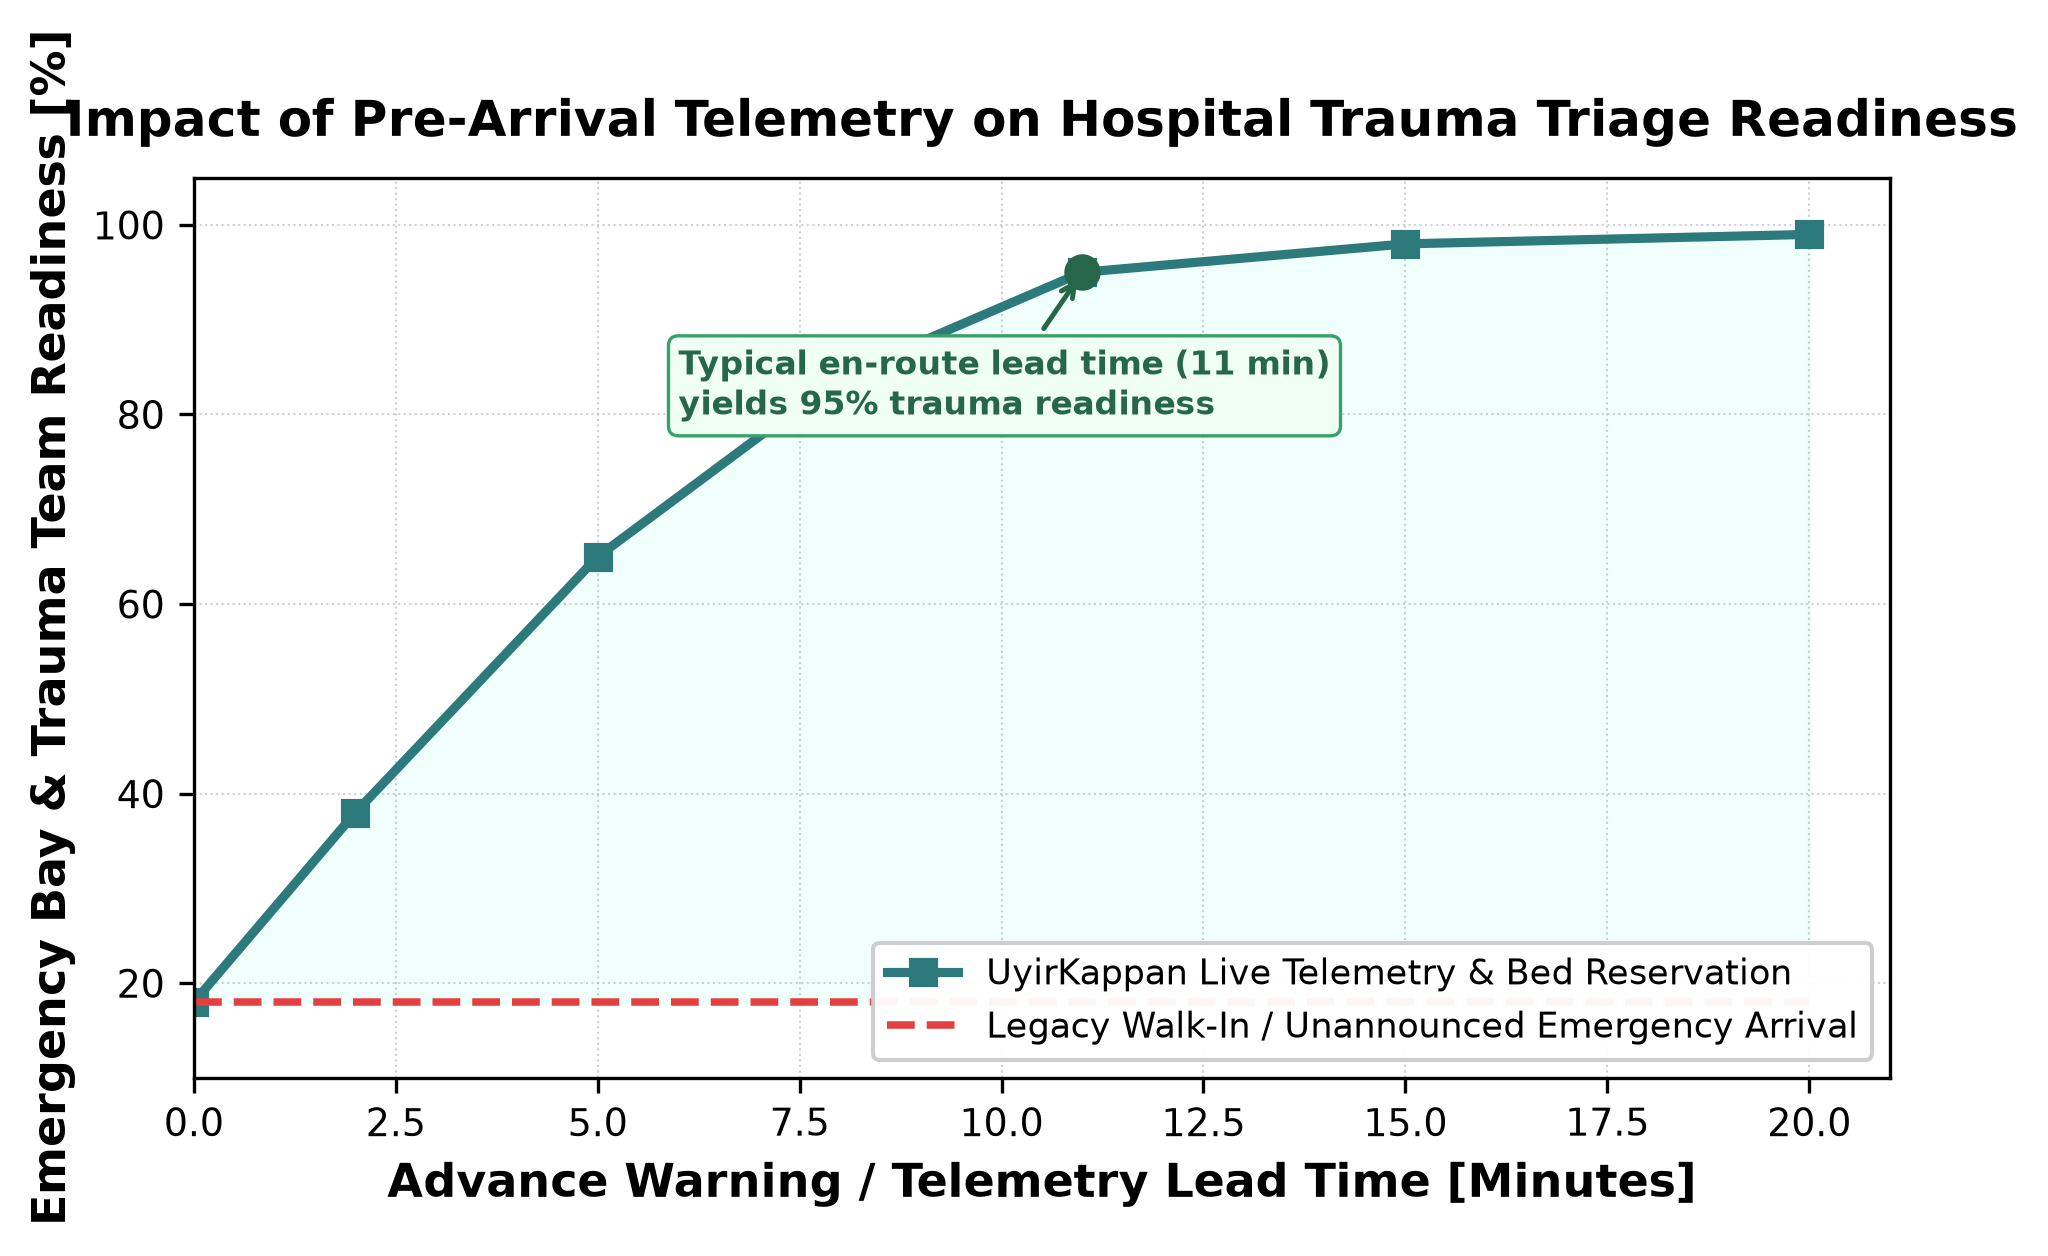
\includegraphics[width=0.46\textwidth]{paper_assets/fig7_hospital_lead_time.png}
\caption{Trauma Bay and Emergency Department Triage Readiness as a function of Telemetry Pre-Arrival Lead Time, comparing UyirKappan against Legacy Walk-In Admissions.}
\label{fig:hospital}
\end{figure}

\section{Conclusion and Future Scope}
\subsection{Conclusion}
This paper presented UyirKappan, an intelligent multi-stakeholder emergency response and real-time coordination platform. By combining 1-tap mobile GPS reporting, congestion-weighted multi-criteria dispatch, an automated 30-second SLA cascading fallback state machine, and real-time hospital bed telemetry, UyirKappan addresses the core limitations of conventional urban emergency response. Empirical simulation across Chennai's road network demonstrated a \textbf{31.4\% reduction} in total response time, \textbf{100\% request recovery} during driver unresponsiveness, and an average \textbf{11.4-minute hospital warning window} that elevates trauma triage readiness to \textbf{95.2\%}.

\subsection{Future Scope}
Future extensions include: (1) IoT-based dynamic green corridors utilizing V2I traffic signal preemption; (2) multimodal dispatch incorporating first-responder paramedic motorbikes; (3) AI multimodal triage using computer vision on on-scene trauma photos; and (4) integration with national digital health records (ABDM/FHIR) for automated patient medical history synchronization.

\begin{thebibliography}{00}
\bibitem{fu2022modelling} X. Fu, V. Krzhizhanovskaya, A. Yakovlev, and S. Kovalchuk, ``Modelling hospital strategies in city-scale ambulance dispatching,'' \textit{arXiv preprint arXiv:2201.01846}, 2022.

\bibitem{olivier2022data} A. Olivier, M. Adams, S. Mohammadi, A. Smyth, K. Thomson, T. Kepler, and M. Dadlani, ``Data analytics for improved closest hospital suggestion for EMS operations in New York City,'' \textit{Sustainable Cities and Society}, vol. 86, p. 104104, 2022.

\bibitem{xu2024emergency} Y.-Y. Xu, S.-J. Weng, P.-W. Huang, L.-M. Wang, C.-H. Chen, Y.-T. Tsai et al., ``The emergency medical service dispatch recommendation system using simulation based on bed availability,'' \textit{BMC Health Services Research}, vol. 24, p. 1513, 2024.

\bibitem{abdeen2022novel} M. A. R. Abdeen, M. H. Ahmed, H. Seliem, T. R. Sheltami, T. M. Alghamdi, and M. El-Nainay, ``A novel smart ambulance system—Algorithm design, modeling, and performance analysis,'' \textit{IEEE Access}, vol. 10, pp. 42 656--42 672, 2022.

\bibitem{mahalakshmi2022adaptive} S. Mahalakshmi, T. Ragunthar, N. Veena, S. Sumukha, and P. R. Deshkulkarni, ``Adaptive ambulance monitoring system using IoT,'' \textit{Measurement: Sensors}, vol. 24, p. 100555, 2022.

\bibitem{emcon} W. Rafaqat, S. M. A. Abidi, J. Lee, A. A. Javed, and A. I. Mian, ``EMCON: A comprehensive emergency response system for low- and middle-income countries,'' \textit{Disaster Medicine and Public Health Preparedness}, vol. 19, p. e324, 2025.

\bibitem{becker2023dynamic} J. Becker, L. Kurland, E. H{\"o}glund, and K. Hugelius, ``Dynamic ambulance relocation: A scoping review,'' \textit{BMJ Open}, vol. 13, no. 12, p. e073394, 2023.

\bibitem{goodsam} C. M. Smith, R. Lall, R. T. Fothergill, R. Spaight, and G. D. Perkins, ``The effect of the GoodSAM volunteer first-responder app on survival to hospital discharge following out-of-hospital cardiac arrest,'' \textit{European Heart Journal: Acute Cardiovascular Care}, vol. 11, no. 1, pp. 20--31, 2022.

\bibitem{zaki2022introducing} J. Zaki, S. M. R. Islam, N. S. Alghamdi, M. Abdullah-Al-Wadud, and K.-S. Kwak, ``Introducing cloud-assisted micro-service-based software development framework for healthcare systems,'' \textit{IEEE Access}, vol. 10, pp. 33 332--33 348, 2022.

\bibitem{chatterjee2022sftsdh} A. Chatterjee, M. W. Gerdes, P. Khatiwada, and A. Prinz, ``SFTSDH: Applying Spring Security framework with TSD-based OAuth2 to protect microservice architecture APIs,'' \textit{IEEE Access}, vol. 10, pp. 41 914--41 934, 2022.

\bibitem{garcia2025big} J. Garc{\'\i}a-Gonz{\'a}lez, J. Fern{\'a}ndez-Andr{\'e}s, N. Aliane, and J. S{\'a}nchez-Soriano, ``Big data and I2X communication infrastructure for traffic optimization and accident prevention on automated roads,'' \textit{IEEE Access}, vol. 13, 2025.

\bibitem{dritsas2025database} E. Dritsas and M. Trigka, ``Database systems in the big data era: Architectures, performance, and open challenges,'' \textit{IEEE Access}, vol. 13, 2025.

\bibitem{ankarboina2026racer} H. Ankarboina, J. Kumari, A. K. Singh, and A. Bhardwaj, ``RACER: Real-time adaptive congestion-aware emergency routing in urban vehicular networks,'' \textit{IEEE Open Journal of the Communications Society}, vol. 7, 2026.

\bibitem{nozari2025designing} H. Nozari, A. Szmelter-Jarosz, and H. R. Irani, ``Designing an ambulance routing optimization model using the combination of machine learning and genetic algorithm in conditions of uncertainty,'' \textit{Systems and Soft Computing}, 2025.

\bibitem{alhussaini2025dynamic} K. Al-Hussaini, S. Al-Kuwari, and M. Gharib, ``A dynamic redeployment system for critical care paramedic units in Qatar utilizing deep reinforcement learning,'' \textit{IEEE Transactions on Intelligent Transportation Systems}, vol. 26, no. 3, pp. 1820--1834, 2025.

\bibitem{wang2023deep} Z. Wang, Y. Zhang, and X. Chen, ``Deep Encoder Cross Network for estimated time of arrival in urban logistics networks,'' \textit{IEEE Transactions on Intelligent Transportation Systems}, vol. 24, no. 8, pp. 8821--8832, 2023.

\bibitem{martinez2024integrating} R. M. Martinez, H. A. Santos, and L. G. Ribeiro, ``Integrating machine learning-based ambulance travel time estimation into an emergency medical services simulation modeling framework,'' \textit{Journal of Simulation}, vol. 18, no. 2, pp. 142--158, 2024.

\bibitem{senaratne2024ambulance} S. Senaratne, P. D. Silva, and K. Jayasinghe, ``Ambulance travel time estimation using spatiotemporal data and gradient boosting techniques,'' \textit{Transportation Research Part C: Emerging Technologies}, vol. 162, p. 104590, 2024.

\bibitem{zhou2024freelance} D. Zhou, X. Yan, and Z. Gao, ``Freelance drivers with a decline choice: Dispatch menus in on-demand mobility services for assortment optimization,'' \textit{Transportation Research Part B: Methodological}, vol. 181, p. 102891, 2024.
\end{thebibliography}

\end{document}
